% warwickthesis.tex modified by M Hadley from utthesis.doc  Sept 96
% Significant changes were made in 2009, first to work seemlessly with pdflatex
% and secondly to use the setspace package to control linespacing -
% removing some incompatibilities that existed before.
% any comments or problems - contact me  <m.j.hadley@warwick.ac.uk>
%%%%%%%%%%%%%%%%%%%%%%%%%%%%%%%%%%%%%%%%%%%%%%%%%%%%%%%%%%%%%%%%%%%%%%%%%%%%%
%%%
%%% File: utthesis.doc, version 2.0, January 1995
%%% =============================================
%%% Copyright (c) 1995 by Dinesh Das.  All rights reserved.
%%% This file is free and can be modified or distributed as long as
%%% you meet the following conditions:
%%%
%%% (1) This copyright notice is kept intact on all modified copies.
%%% (2) If you modify this file, you MUST NOT use the original file name.
%%%
%%% This file contains a template that can be used with the package
%%% utthesis.sty and LaTeX2e to produce a th\citep that meets the requirements
%%% of the Graduate School of The University of Texas at Austin.
%%%
%%% All of the commands defined by utthesis.sty have default values (see
%%% the file
%           warwickthesis.sty
%%%                        for these values).  Thus, theoretically, you
%%% don't need to define values for any of them; you can run this file
%%% through LaTeX2e and produce an acceptable thesis, without any text.
%%% However, you probably want to set at least some of the macros (like
%%% \thesisauthor).  In that case, replace "..." with appropriate values,
%%% and uncomment the line (by removing the leading %'s).
%%%
%%%%%%%%%%%%%%%%%%%%%%%%%%%%%%%%%%%%%%%%%%%%%%%%%%%%%%%%%%%%%%%%%%%%%%%%%%%%%
% all comments starting with %! have been added by M Hadley as
% part of the conversion for the university of warwick
%
%
%\documentclass[11pt,a4paper,twoside]{report}      %% LaTeX2e document.
%%* Removed twoside option which is no longer accepted - you might want to use it for drafts.
\documentclass[11pt,a4paper]{report} 
%\documentclass[11pt,a4paper,draft]{report}     %% LaTeX2e document.
\usepackage{thesis,setspace,graphicx}     %!  setspace is used to control linepacing
\usepackage[round]{natbib}                    %! needed for Harvard style of references.

\usepackage{afterpage} 

\usepackage{boldline} 
%\hlineB bold lines


\usepackage{array}
                                                %! for more notes see the bibliography section below
\usepackage{enumerate}  %! used for the library form, but you might find it useful too.

\usepackage{subfigure} %! subfigures 
\usepackage{mathtools} %! use \MoveEqLeft


\usepackage{tikz}
\usetikzlibrary{matrix,arrows,shapes,snakes, positioning, calc}
\usetikzlibrary{chains,positioning}

\usepackage[font=small,labelfont=bf]{caption}
\usepackage{multirow}
%\multirow{2}{*} { text}

\usepackage{colortbl}
\usepackage{array}
\usepackage{amsmath, mathtools, amssymb, bbm, dsfont}
 
\allowdisplaybreaks %! break equation into two pages


% table width coloumn
\newcolumntype{L}[1]{>{\raggedright\let\newline\\\arraybackslash\hspace{0pt}}m{#1}}
\newcolumntype{C}[1]{>{\centering\let\newline\\\arraybackslash\hspace{0pt}}m{#1}}
\newcolumntype{R}[1]{>{\raggedleft\let\newline\\\arraybackslash\hspace{0pt}}m{#1}}

% larger than \Bigg brackets
\makeatletter
\newcommand{\vast}{\bBigg@{4}}
\newcommand{\Vast}{\bBigg@{5}}
\makeatother

% \mastersthesis                     %% Uncomment one of these; if you don't
% \phdthesis                         %% use either, the default is \phdthesis.

%\thesisdraft                       %% Uncomment this if you want a draft
                                     %% version; this will print a timestamp
                                     %% on each page of your thesis.

% \leftchapter                       %% Uncomment one of these if you want
% \centerchapter                     %% left-justified, centered or
 \rightchapter                      %% right-justified chapter headings.
                                     %% Chapter headings includes the
                                     %% Contents, Acknowledgments, Lists
                                     %% of Tables and Figures and the Vita.
                                     %% The default is \centerchapter.

%\renewcommand{\familydefault}{cmss}  %! removed April 2009 because the default times font reads more easily
                                     %! for larger blocks of text.%!
                                     %! Added March 2003.
                                     %! This alternative is to use a sans serif font as in
                                     %!  the Warwick Corporate style.
                                     %! The default is Times, which is still acceptable.


%\onehalfspacing                      %! This is the default and gives an acceptable "double spaced" thesis
                                     %! It is the minimum spacing accepted by the graduate school, and there is no reason to increase the spacing.
% \singlespacing                     %! Uncomment if you want single-spacing,
\doublespacing                     %! uncomment if you want real double-spacing for some perverse reason.

%\setlength{\textheight}{9.0in}      %! Uncomment this for a slightly
                                     %! longer page. The default is now 8.5in (from Feb 2010)
                                     %! regulations require page numbers to be at least 1.5cm into the page.
                                     %! You can even try a longer page to save paper.

%! Double sided printing is no longer allowed (March 2008), it caused too many problems at binding,
                              %\setlength{\evensidemargin}{0.15in}  %! Uncomment this line for double sided printing
                                      %! Double-sided printing has recently been
                                      %! allowed by the Graduate School (March 2003)
                                      %! The default is {0.7in} for single sided.
%! Double sided printing is no longer allowed (March 2008), it caused too many problems at binding,

\renewcommand{\thesisdepartmentname}{Nuffield Department of Population Health}    %! The name of
                                                  %   the department

%! \renewcommand{\thesissubmission}{Submitted to the University of Warwick\\
%!              in partial fulfilment of the whererequirements\\
%!                   for admission to the degree of\\}
%!
%!!!!!!!! default is:
%!
\renewcommand{\thesissubmission}{Submitted to the University of Oxford\\
                        for the degree of}
%!
%! In the title page this wording will be preceeded by:  thesis\\
%!                 and ended by:  Doctor of Philosophy   (or the
%!                                               selected alternative names
%! use \\ where you want a new line

\renewcommand{\thesisauthor} {Alexander Bowring}    %% Your official name.
\renewcommand{\thesisauthorno}{1139660}  %! your university number, used on the library copyright page.


\renewcommand{\thesismonth}{October}     %% Your month of graduation.

\renewcommand{\thesisyear}{2019}      %% Your year of graduation.

\renewcommand{\thesistitle}{On the Reproducibility and Interpretability of Group-Level Task-fMRI Results}     %% The title of your thesis; use
                                     %% mixed-case.

%! \renewcommand{\thesistitletypesize}{\LARGE}   %! Put this in if you
                                  %!   want a Large title the default is \large

\renewcommand{\thesisauthorpreviousdegrees}{....}
                                     %% Your previous degrees, abbreviated;
                                     %% separate multiple degrees by commas.

\renewcommand{\thesissupervisor}{Thomas E Nichols}
                                     %% Your thesis supervisor; use mixed-case
                                     %% and don't use any titles or degrees.

\renewcommand{\thesisauthoraddress}{....}
                                     %% Your permanent address; use "\\" for
                                     %% linebreaks.
%%%%%%%%%%%%%%%%%%%%%%%%%%%%%%%%%%%
%! For the library declaration page only
%! \renewcommand{\thesiscopyrightagree}{agree}
                        %! agreement to allow single photocopies this is the default
%! \renewcommand{\thesiscopyrightagree}{do not agree}
                        %! refusal  to allow single photocopies

%! \renewcommand{\thesiscopyrightagreewhen}{immediately.}
                        %! that is the default to be used in all but the most exceptional circumstances
%! \renewcommand{\thesiscopyrightagreewhen}{after an embargo period of ……….................... months/years as agreed by the Chair of the Board of Graduate Studies.}
                         %! An alternative, if you have permission. Replace the .... month/years with approved period or change the wording to insert a date.

%! \renewcommand{\thesisinternetagree}{thesis can be made publicly available online.}
                         %! default online declaration for WRAP
%! \renewcommand{\thesisinternetagree}{thesis cannot be made publicly available online.}
                          %! use if necessary
%! \renewcommand{\thesisinternetagree}{thesis can be made publicly available only after…..}
                          %! conditional agreement, please put the date in place of the dots, ending with a fullstop.
%! \renewcommand{\thesisinternetagree}{full thesis cannot be made publicly available online, but I am submitting a separately identified additional abridged version that can be made available online.}



%%%%%%%%%%%%%%%%%%%%%%%%%%%%%%%%%%%%%%%%%%%%%%%%%%%%%%%%%%%%%%%%%%%%%%%%%%%%%
%%%
%%% The following commands are all optional, but useful if your requirements
%%% are different from the default values in utthesis.sty.  To use them,
%%% simply uncomment (remove the leading %) the line(s).

% \renewcommand{\thesisdegree}{...}  %% Uncomment this only if your thesis
                                     %% degree is NOT "DOCTOR OF PHILOSOPHY"
                                     %% for \phdthesis or "MASTER OF ARTS"
                                     %% for \mastersthesis.  Provide the
                                     %% correct FULL OFFICIAL name of
                                     %% the degree.

% \renewcommand{\thesisdegreeabbreviation}{...}
                                     %% Use this if you also use the above
                                     %% command; provide the OFFICIAL
                                     %% abbreviation of your thesis degree.

%\renewcommand{\thesistype}{Thesis}    %% Use this ONLY if your thesis type
                                     %! is NOT "Thesis"
                                     %% Provide the OFFICIAL type of the
                                     %% thesis; use mixed-case.

% \renewcommand{\thesistypist}{...}  %% Use this to specify the name of
                                     %% the thesis typist if it is anything
                                     %% other than "the author".

%%%
%%%%%%%%%%%%%%%%%%%%%%%%%%%%%%%%%%%%%%%%%%%%%%%%%%%%%%%%%%%%%%%%%%%%%%%%%%%%%


%%%% My Packages

\usepackage{latexsym,amsmath,amssymb,amsfonts,lineno,xcolor}
\usepackage{graphicx,color,epsfig,fancyhdr}
\usepackage{mathrsfs,bbm,dsfont}
\usepackage{fancyhdr}
\usepackage{array}
\usepackage{subfigure}
%\newtheorem{def}{Definition}
\usepackage{multirow}
\usepackage{amssymb}% http://ctan.org/pkg/amssymb
\usepackage{pifont}% http://ctan.org/pkg/pifont
\usepackage{bbding}
\usepackage{bm}

\usepackage{adjustbox}

\usepackage{colortbl}
\usepackage[round]{natbib}


\usepackage{textcomp}
% Color for the links, references and other parts if needed
\usepackage[colorlinks=true,linkcolor=blue]{hyperref}
\usepackage{color}
\definecolor{colorlink}{rgb}{0, 0, .6}  % dark blue
\definecolor{colornew}{rgb}{0, .35, 0}  % dark green
\hypersetup{colorlinks=true,citecolor=colorlink,filecolor=colorlink,linkcolor=colorlink,urlcolor=colorlink}

\graphicspath{{Figures/}{Figures/SC_Supplementary_Figs}}

%%Habib's modifications
\newcommand{\cov}{\mathrm{cov}}
\newcommand{\tr}{\mathrm{tr}}
\newcommand{\corr}{\mathrm{corr}}
\newcommand{\var}{\mathrm{var}}
%%%%

%\input header.tex          %! Input declarations, new
                              %theorems etc.

%% ALEX's Modifications
% Change default text to Lato
\usepackage[T1]{fontenc}
\usepackage[default]{lato}
\DeclareMathOperator*{\argmin}{arg\,min}

% Change chapter style
\usepackage{titlesec}
\titleformat{\chapter}[display]
  {\Large}
  {\filleft\MakeUppercase{\chaptertitlename} \Huge\thechapter}
  {1ex}
  {\titlerule\vspace{1ex}\filleft}[\vspace{1ex}\titlerule]


% Gobble page numbers for large figures
\usepackage{floatpag}

% Landscape figures
\usepackage{rotating}

% booktabs for tables
\usepackage{booktabs}

% Allow long tables
\usepackage{longtable}

% Allow 'Three part table', caption above and below, used for software processing steps in SC 
\usepackage[flushleft]{threeparttable}


% Contour Inference operators
\DeclareMathOperator{\Ac}{\mathcal{A}_{c}}
\DeclareMathOperator{\Ahatc}{\hat{\mathcal{A}}_{c}}
\DeclareMathOperator{\Ahatcp}{\hat{\mathcal{A}}_{c}^+}
\DeclareMathOperator{\Ahatcm}{\hat{\mathcal{A}}_{c}^{\textrm{--}}}
\DeclareMathOperator{\dAc}{\partial\mathcal{A}_{c}}
\DeclareMathOperator{\dAhatc}{\partial\hat{\mathcal{A}}_{c}}
\DeclareMathOperator{\sigmahat}{\hat{\sigma}}
\DeclareMathOperator{\Xbar}{\bar{X}}
\DeclareMathOperator{\arcsinh}{arcsinh}
\DeclareMathOperator{\Mbar}{\bar{\mathcal{M}}}
\DeclareMathOperator{\Acmu}{\mathcal{A}_{c,\mu}}
\DeclareMathOperator{\Ahatcpm}{\hat{\mathcal{A}}_{c}^\pm}
\DeclareMathOperator{\Ahatcpmu}{\hat{\mathcal{A}}_{c,\mu}^+}
\DeclareMathOperator{\Ahatcpd}{\hat{\mathcal{A}}_{c,\textit{d}}^+}
\DeclareMathOperator{\Ahatcmmu}{\hat{\mathcal{A}}_{c,\mu}^{\textrm{--}}}
\DeclareMathOperator{\Ahatcmd}{\hat{\mathcal{A}}_{c,\textit{d}}^{\textrm{--}}}
\DeclareMathOperator{\dAcmu}{\partial\mathcal{A}_{c,\mu}}
\DeclareMathOperator{\Cov}{\mathrm{Cov}}
\DeclareMathOperator*{\E}{\mathbb{E}}

% Package for the 'moon' symbol used in the 1D intuition figure for %BOLD CSs.
\usepackage{wasysym}

% Package for the proof in the Cohens D chaper
\usepackage{amsthm}

\begin{document}

%\thesiscopyrightpage                 %! Generate the copyright page for the library.
%%%%%%%%%%% \thesiscopyrightpagehardcopyonly This only applies for a masters thesis that will not go online.

%%* Uncomment a ttitle page.
 \thesistitlepage                     %% Generate the title page.
%\thesistitlecolourpage           %! Generates a COLOUR title page.


\pagenumbering{gobble}
\begin{singlespace}
\begin{thesisabstract}
\begin{singlespace}
In this thesis, we aim to address two topical issues at the forefront of task-based functional magnetic resonance imaging (fMRI). The first of these is a growing apprehension within the field about the reproducibility of findings that make up the neuroimaging literature. To confront this, we assess how the choice of software package for analyzing fMRI data can impact the final group-level results of a neuroimaging study. We reanalyze data from three published task-fMRI studies within the three most widely-used neuroimaging software packages -- AFNI, FSL, and SPM -- and then apply a range of comparison methods to gauge the scale of variability across the results. While qualitatively we find similarities, our quantitative assessment methods discover considerable differences between the final statistical images obtained with each package. Ultimately, we conclude that exceedingly weak effects may not generalize across fMRI analysis software. 

In the second part of this work we shift our attention to the analytical methods applied for fMRI inference. Here, we seek to overcome limitations with the traditional statistical approach, where for sufficiently large data sizes current methods determine universal activation across the brain, rendering the results as uninterpretable. We extend on a method proposed by \citet*{Sommerfeld2018-zl} (\textit{SSS}) to develop spatial Confidence Sets (CSs) on clusters found in thresholded raw blood-oxygen-level-dependent (BOLD) effect size maps. The CSs give statements on the locations where raw effect sizes exceed, and fall short of, a purposeful \textit{non-zero} threshold. We propose several theoretical and practical implementation advancements to the original method formulated in \textit{SSS}, delivering a procedure with superior performance in sample sizes as low as $N = 60$. We validate the method with 3D Monte Carlo simulations that resemble fMRI data. We then compute CSs for the Human Connectome Project (HCP) working memory task contrast images, illustrating the brain regions that show a reliable \%BOLD for a given \%BOLD threshold. 

In the final part of this thesis, we develop the CSs to operate on standardized Cohen's $d$ effect size images. We derive the statistical properties of the Cohen's $d$ estimator to motivate three algorithms for computing Cohen's $d$ CSs, including a novel method based on normalizing the distribution of Cohen's $d$. With intensive 3D Monte Carlo simulations, we find that two of these methods can be effectively applied to fMRI data. We compute Cohen's $d$ CSs on the HCP data, and by comparing the CSs with results obtained from a standard testing procedure, exemplify the improved localization of effects that can be gained by using the Confidence Sets. 

%%Over the last three decades, Functional Magnetic Resonance Imaging  has rapidly progressed to become the primary tool for human brain mapping. Recently however, considerable attention within the field has been directed towards data-sharing and open science initiatives. This has been driven by a growing apprehension about the reproducibility of findings that constitute the neuroimaging literature, amid concerns that current inference procedures are often misused or misinterpreted such that the overall scientific conclusions become distorted. One aspect specific to neuroimaging pinpointed as a cause for poor reproducibility is the high flexibility of a typical fMRI workflow. In the first part of this thesis, we investigate how the choice of software package used to conduct a statistical analysis can influence the group-level results of a task-fMRI study. We use publicly shared data from three published task-fMRI studies, and reanalyze each study within the three main neuroimaging software packages, AFNI, FSL and SPM, using parameteric and nonparametric inference. All information on how to process, analyze, and model each dataset we obtain from the publications. We use a variety of quantitative and qualitative comparison methods to gauge the scale of variability in our results and assess fundamental differences between each software package. While qualitatively we find broad similarities between packages, we also discover marked differences, such as Dice similarity coefficient values ranging from 0.000 to 0.743 in comparisons of thresholded statistic maps between software. We discuss the challenges involved in our replication attempt, while also utilizing open science tools in an effort to make our own research reproducible. In the second part of this thesis, we extend a contour inference method initially proposed by \citet*{Sommerfeld2018-zl} \textit{SSS} to develop spatial confidence sets (CSs) on clusters found in thresholded blood-oxygen-level dependent (BOLD) effect size maps. While traditional inferences based on hypothesis testing indicate where the null, i.e. an effect size of zero, can be rejected, the CSs give statements about where effect sizes exceed a \textit{positive} threshold analogous to confidence intervals simultaneously across the entire brain. We make advancements to theoretical aspects and implementation of contour inference to improve the method's finite-sample performance. We extend the wild bootstrap theory presented in \textit{SSS}, proposing a method based on the t-bootstrap, and recommend that the bootstrapped residuals are multiplied by Rademacher variables instead of Gaussian variables. We also develop a linear interpolation method for computing the topological boundary over which the bootstrap is applied. Notably, we demonstrate that the framework used in \textit{SSS} for assessing simulations manifests considerable positive bias in the simulation results, and propose our own novel construction to solve this issue. In the final part of this thesis, we make further theoretical developments to contour inference so that the method can operate on the Cohen's \textit{d} and partial $R^{2}$ effect sizes commonly reported at the end of a neuroimaging study. For the second and third parts of this thesis, we carry out intensive Monte Carlo simulations on synthetic 3D data to investigate the accuracy of contour inference on signals representative of fMRI activation clusters. We also demonstrate the method on two `big' fMRI datasets, obtaining confidence sets to localize activation in functional data from the Human Connectome Project and UK Biobank.	

%With increasing availability to population-size neuroimaging databases, the limitations of such inference methods are also %becoming apparent: with sufficient statistical power, the null-hypothesis of no activation can be rejected over essentially the %entire brain.  
\end{singlespace}
\end{thesisabstract}
\end{singlespace}


%%* Start roman page numbering here for , etc
\pagenumbering{roman} %! Begins roman numerals start from page i.

\begin{thesisacknowledgments}        %% Use this to write your
%  \input ack.tex                    %% acknowledgments; it can be anything
                                     %% allowed in LaTeX2e par-mode.
                                     %! This following is not needed, but you may like to add it.
%This \lowercase\expandafter{\thesistype} was typeset with
%\LaTeXe\footnote{\LaTeXe{} is an extension of \LaTeX. \LaTeX{} is
%a collection of macros for \TeX. \TeX{} is a trademark of the
%American Mathematical Society. The style package {\em warwickthesis} was
%used.} by \thesistypist.

\end{thesisacknowledgments}

\begin{thesisdeclaration}        
I, Alexander Bowring, hereby declare that except where specific reference is made to the work of others, the content of this thesis is original and has not been submitted in whole or in part for consideration for any other degree or qualification in these, or any other universities. This thesis is the result of my own work and includes nothing which is the outcome of work done in collaboration, except where specifically indicated in the text.

\begin{itemize}
\item The work presented in Chapter 3 has been published in the \textit{Human Brain Mapping} journal, \citet*{Bowring2019-fc}. This work was presented at the \textit{Organization for Human Brain Mapping} (OHBM) Annual Meetings in 2017 and 2018. At the OHBM 2018 Annual Meeting, this work was the recipient of an oral presentation and a Merit Abstract Award. 
 
\item The work presented in Chapter 4 has been published in the \textit{NeuroImage} journal \citet*{BOWRING2019116187}. This work was presented at the OHBM Annual Meeting in 2017, where it was the recipient of an oral presentation. 

\item The work presented in Chapter 5 will shortly be submitted for publication.
\end{itemize}

\vspace{2cm}
\hspace{-1.2cm}
Alexander Bowring 

\hspace{-1.2cm}
September 2019

\tableofcontents                     %% Generate table of contents.
% \listoftables                      %% Uncomment this to generate list
                                     %% of tables.
% \listoffigures                     %% Uncomment this to generate list
                                     %% of figures.

%For detailed list of publications, please see Appendix \ref{app:LP}.



%! Use this to declare the extent of
                 %! the original work,
                 %! collaboration, other published
                                 %! material etc.it can be anything
                                 %% allowed in LaTeX2e par-mode.


\end{thesisdeclaration}


%\begin{thesisabstract}               %% Use this to write your thesis
%                                     %% abstract; it can be anything
%                                     %% allowed in LaTeX2e par-mode.
%%!  \begin{singlespace}       %! uncomment this if you need single spacing
%%   \input abstract.tex       %!           don't forget the end spacing!
%                                     %! It must fit on one page.
%                                     %! single spacing and smaller
%                                     %! font size
%                                     %!  is allowed here.
%%!   \end{singlespace}
%

%\begin{thesisabbreviations}       %! Use this to give a list of
                                   %! abbreviateons
                                   %! It can be anything
%\end{thesisabbreviations}         %! allowed in LaTeX2e par-mode.
                                   %!The following may be useful':
                     %!\begin{itemize}
                     %!     \item[symbol]descriptive text..
                     %!\end{itemize}

%\end{thesisabbreviations}
%!!!!!!!!!!!!!!!                     %% Begin your thesis text here; follow
                                     %% the report style and group your text
                                     %% in chapters, sections, etc. eg:
%%* don't need this with one-sided printing
%\newpage{\pagestyle{empty}\cleardoublepage} %! ensure that Chapter 1 starts on an odd
                                           %! page when using double sided printing.
%%* Start arabic numbering of main text here
\pagenumbering{arabic} %! Begins arabic numerals start from page 1.


\chapter{Introduction}
\label{chap:introduction_chapter}
%You would usually put the main content in separate files.
\input introduction.tex

\chapter{Background}
\label{chap:background}
\input Background.tex

\chapter{Exploring the Impact of Analysis Software on Task-fMRI Results}
\label{chap:software}
\input Software_Comparison.tex

\chapter{Spatial Confidence Sets for Raw Effect Size Images}
\label{chap:BOLD}
\input Contour.tex

\chapter{Spatial Confidence Sets for Cohen's \textit{d} Effect Size Images}
\label{chap:cohen}
\input Cohen.tex
 
\chapter{Conclusion and Future Work}
\label{chap:conclusion}
\input Conclusion.tex
%\input Conc.tex
%% More chapters.
%!
%! There are a few variations of reference
%\begin{verbatim}\citet[chap. 2]{ballentine82}|
%\end{verbatim}
%for a textual one, as \citet[chap. 2]{ballentine82}.\\
% \\
%\begin{verbatim}\citep{abraham_etal}
% \end{verbatim}
% for a parenthetical citation \citep{abraham_etal},\\
%
% \begin{verbatim}\citep*{MTW}
% \end{verbatim}
% for a full list of authors use a * parenthetical citation \citep*{MTW},\\
% \\
%!!!!!!!!!!!!!!!

\appendix                            %% this will do the appendices
\chapter{Software Comparison Supplementary Material}
%\documentclass{article}   	% use "amsart" instead of "article" for AMSLaTeX format
%\usepackage[margin=0.5in]{geometry}                		% See geometry.pdf to learn the layout options. There are lots.
%\geometry{letterpaper}                   		% ... or a4paper or a5paper or ... 
%\geometry{landscape}                		% Activate for rotated page geometry
%\usepackage[parfill]{parskip}    		% Activate to begin paragraphs with an empty line rather than an indent
%\usepackage{graphicx}				% Use pdf, png, jpg, or eps§ with pdflatex use eps in DVI mode
								% TeX will automatically convert eps --> pdf in pdflatex
%\usepackage[backend=biber,style=authoryear]{biblatex}
%\addbibresource{appendix.bib}
%\renewcommand*{\nameyeardelim}{\addcomma\space}

%\usepackage{amsthm}
%\usepackage{amsopn}
%\usepackage{amsmath}
%\usepackage{bm}

%\title{Appendix}

%\begin{document}
%\date{\vspace{-5ex}}
%\maketitle

\section{Percentage BOLD change Maps}
\label{App:SC_supplementary_BOLD}

While each of the three software packages provide contrast of parameter estimate maps (going forth ``contrast estimate''), the units of the analysis differs between software.  We first review the issue of units for fMRI, before detailing how we addressed this issue for each software package.

Raw fMRI data has arbitrary units, and a normalization step is required to produce effect estimates that are both comparable across subjects and give an interpretable magnitude of the BOLD effect. The final units of the contrast estimates depend on how the data, design matrix and contrast vectors are scaled.

Consider arbitrary first level data at a voxel $\bm{Y}$ ($N$-vector) and an fMRI design matrix $\bm{X}$ ($N\times P$ matrix), related by $\mathrm{E}(\bm{Y})=\bm{X}\bm{\beta}$, where $\bm{\beta}$ ($P$-vector) are the regression coefficients and the effect of interest is $\bm{c}\hat{\bm{\beta}}$, where $\bm{c}$ ($P$-row-vector) is the contrast.  The following scaling is needed to ensure interpretable contrasts of parameter estimates.

\begin{itemize}
\item {\bf Data}: The data needs to be scaled so that 1 unit change corresponds to 1\% BOLD change, 
\begin{equation}
\label{eq:SC_sup_data_scale}
\bm{Y}^{*} = \frac{100}{B} \bm{Y}
\end{equation}
where $B$ is an estimate of the mean or baseline.
\item {\bf Design}:  The design needs to be scaled such that a unit change in a coefficient gives rise to a unit effect change in the fitted data, 
\begin{equation}
\label{eq:SC_sup_design_scale}
\bm{X}^{*} = \frac{1}{h} \bm{X}
\end{equation}
where $h$ is the (assumed common) predictor baseline-to-peak (or baseline-to-plateau for long blocks).
\item {\bf Contrast}: The contrast needs to be scaled to preserve the units of the coefficients, 
\begin{equation}
\label{eq:SC_sup_contrast_scale}
\bm{c}^*=\frac{1}{s}\bm{c},
\end{equation}
where $s$ is the sum of the positive contrast elements (or, if all elements are less than zero, minus the sum of the negative elements).
\end{itemize}

  The ideally scaled data, design and contrast gives rise to the contrast estimate $\bm{c}^*\hat{\bm{\beta}}^*$ which we can relate to the arbitrarily scaled data:
\begin{eqnarray}
\label{eq:SC_sup_ideal_scale}
\bm{c}^*\hat{\bm{\beta}}^* &=& \bm{c}^*(\bm{X}^{*\top}\bm{X}^*)^{-1}\bm{X}^{*\top}\bm{Y}^* \notag\\
                          &=& \frac{100h}{Bp}\bm{c}(\bm{X}^{\top}\bm{X})^{-1}\bm{X}^{\top}\bm{Y} \notag\\
                          &=& \frac{100h}{Bp}\bm{c}\hat{\bm{\beta}}.
\end{eqnarray}
This scaling is described in terms of first-level models, but can be applied to a second-level contrast estimate if the values of $h$, $B$ and $p$ are the same for all subjects.

In AFNI, a localized (i.e.\ voxelwise) approach is taken to overcome this hurdle \citep{Chen2017-sb}. By including the `scale' block in our subject-level analysis scripts, each voxel's time series was normalized (in our notation, using a voxelwise $B$) to a voxelwise mean of 100 for all subjects. Scaling of the design matrix is conducted implicitly within AFNI, and as the sum of the contrast elements was 1 in all our analyses, no contrast scaling was necessary. Because of this, the effect estimate maps obtained at the group-level in our AFNI analyses could be directly interpreted as percentage BOLD change maps. 

In FSL and SPM a global (i.e.\ brain-wide) approach is taken for data scaling, so that the modelled data ($\bm{Y}$) has a typical mean value of $B=100$ for SPM, and $B=10,000$ for FSL. In practise, it is known that SPM can underestimate the global mean intensities of each subject, leading to a grand mean intensity \textit{larger} than 100 \citep{Nichols2012-rx}. To account for this, in SPM we calculated $B$ empirically by computing the mean image of all subject-level functional maps and then finding the median value over subjects.  We computed $h$ directly for the block design (ds000109) and based on an isolated event for the event-related design (ds00001); in FSL this required creating dummy designs with high-pass filtering disabled.  Contrast scaling was only required in SPM ($s=3$ for ds000001's 3-run design, $s=2$ for ds000109's 2-run design).



\pagebreak

\section{Partial $R^{2}$ Maps}
\label{App:SC_supplementary_R2}

Since ds000120 used a sine basis HRF, this study's general linear model contained multiple predictor variables which hampered the computation of a percent BOLD change measure.  Instead we computed partial $R^{2}$ maps to assess the explained variance (relative to data variance not already explained by other terms) of the main effect of the saccade condition.

With $\nu_{1}$ and $\nu_{2}$ as the numerator and denominator degrees of freedom of the $F$-statistic, respectively, we used the relationship between $R^{2}$ and the $F$-statistic given by the identity:
%
\begin{equation}
\label{eq:SC_sup_F_to_R}
F = \frac{R^2}{1-R^2}  \frac{\nu_2}{\nu_1},
\end{equation}
%
which solves for $R^{2}$ as
%
\begin{alignat}{4}\label{eq:SC_sup_R_to_F}
  R^2 =  1 - \frac{1}{1 + \frac{\nu_1}{\nu_2} F}.
\end{alignat}

\pagebreak

\section{Supplementary Figures}
\label{App:SC_supplementary_figures}

\begin{figure}[h!tbp]
\centering
	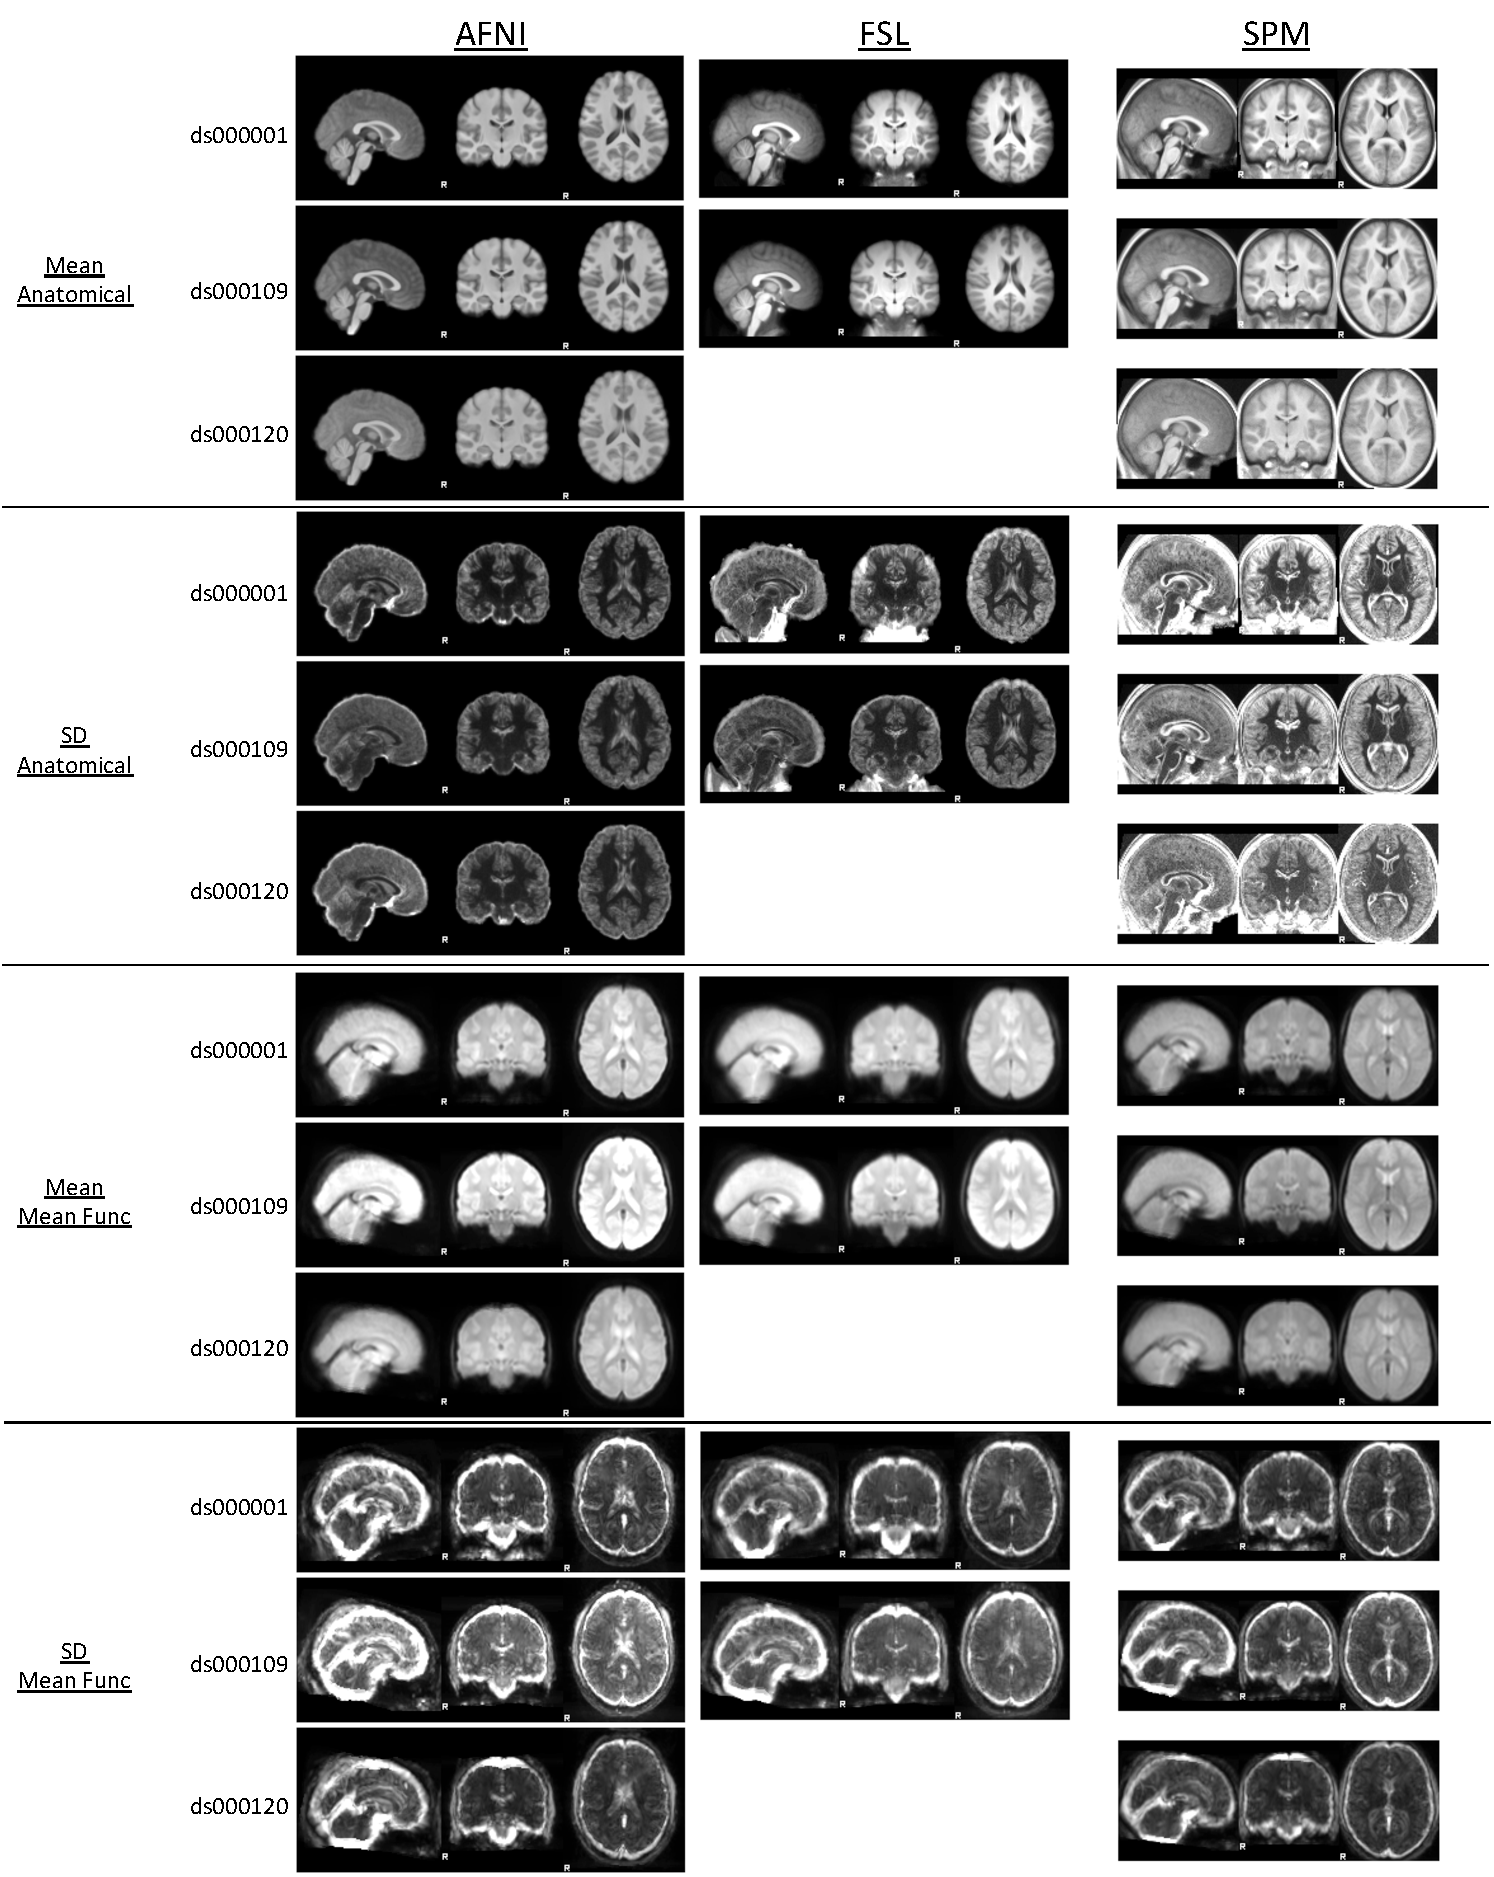
\includegraphics[width=\textwidth]{SC_supp_Registration}	
\caption{Registration Quality Control: Mean and standard deviation of anatomical and mean functional images}
\label{fig:SC_supp_Registration}
\end{figure}

\begin{figure}[htbp]
\centering
	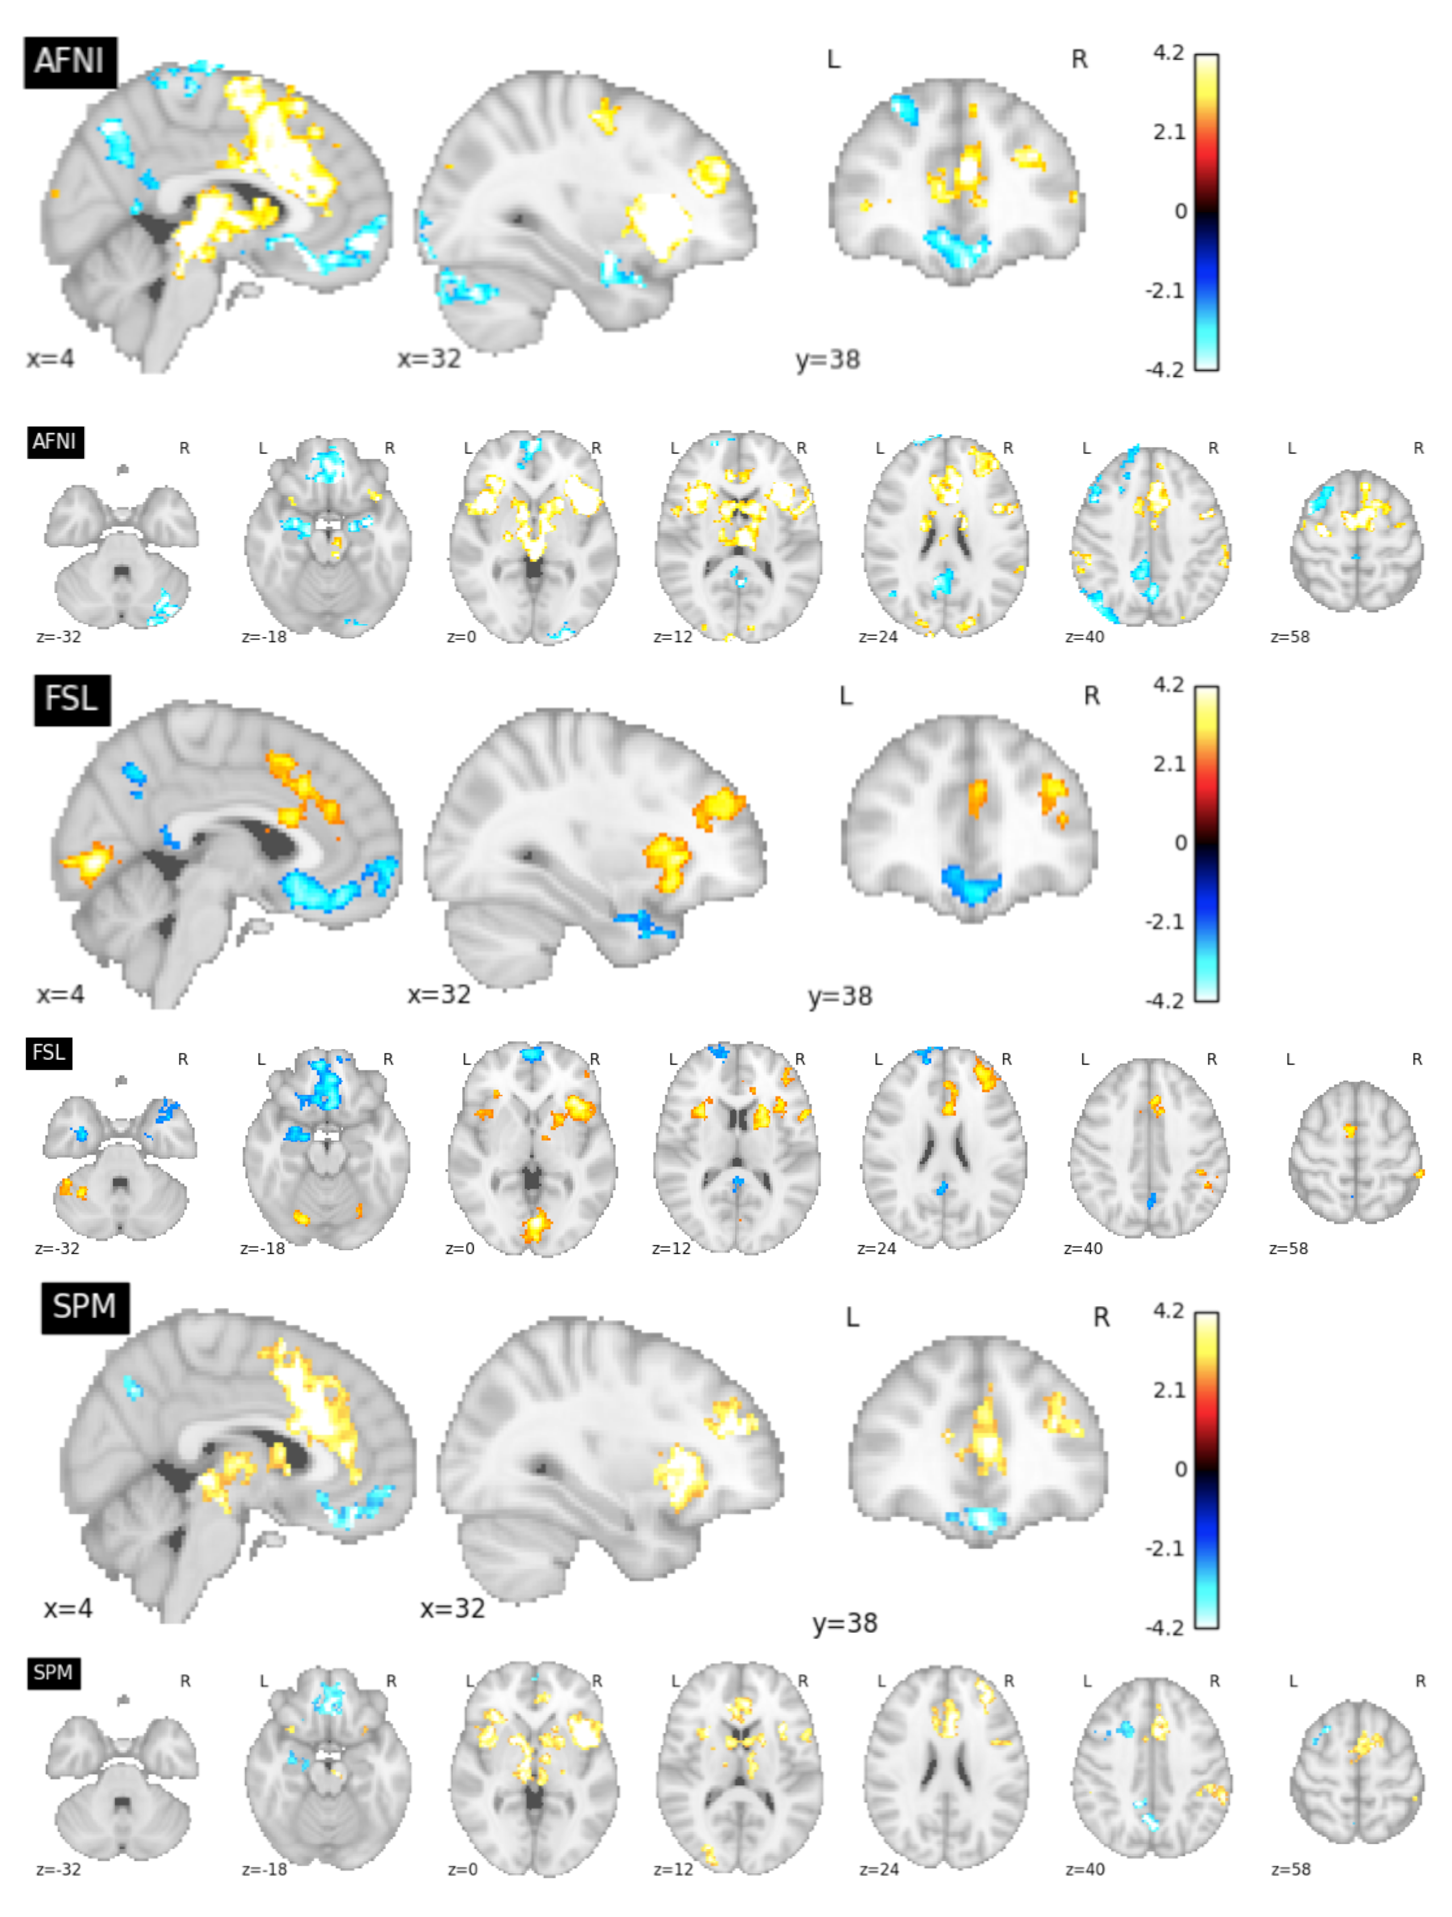
\includegraphics[width=\textwidth]{SC_supp_thresh_ds000001}	
\caption{ds000001 inter-software comparisons, 5\% FWE clusterwise inference}
\label{fig:SC_supp_thresh_ds000001}
\end{figure}

\begin{figure}[htbp]
\centering
	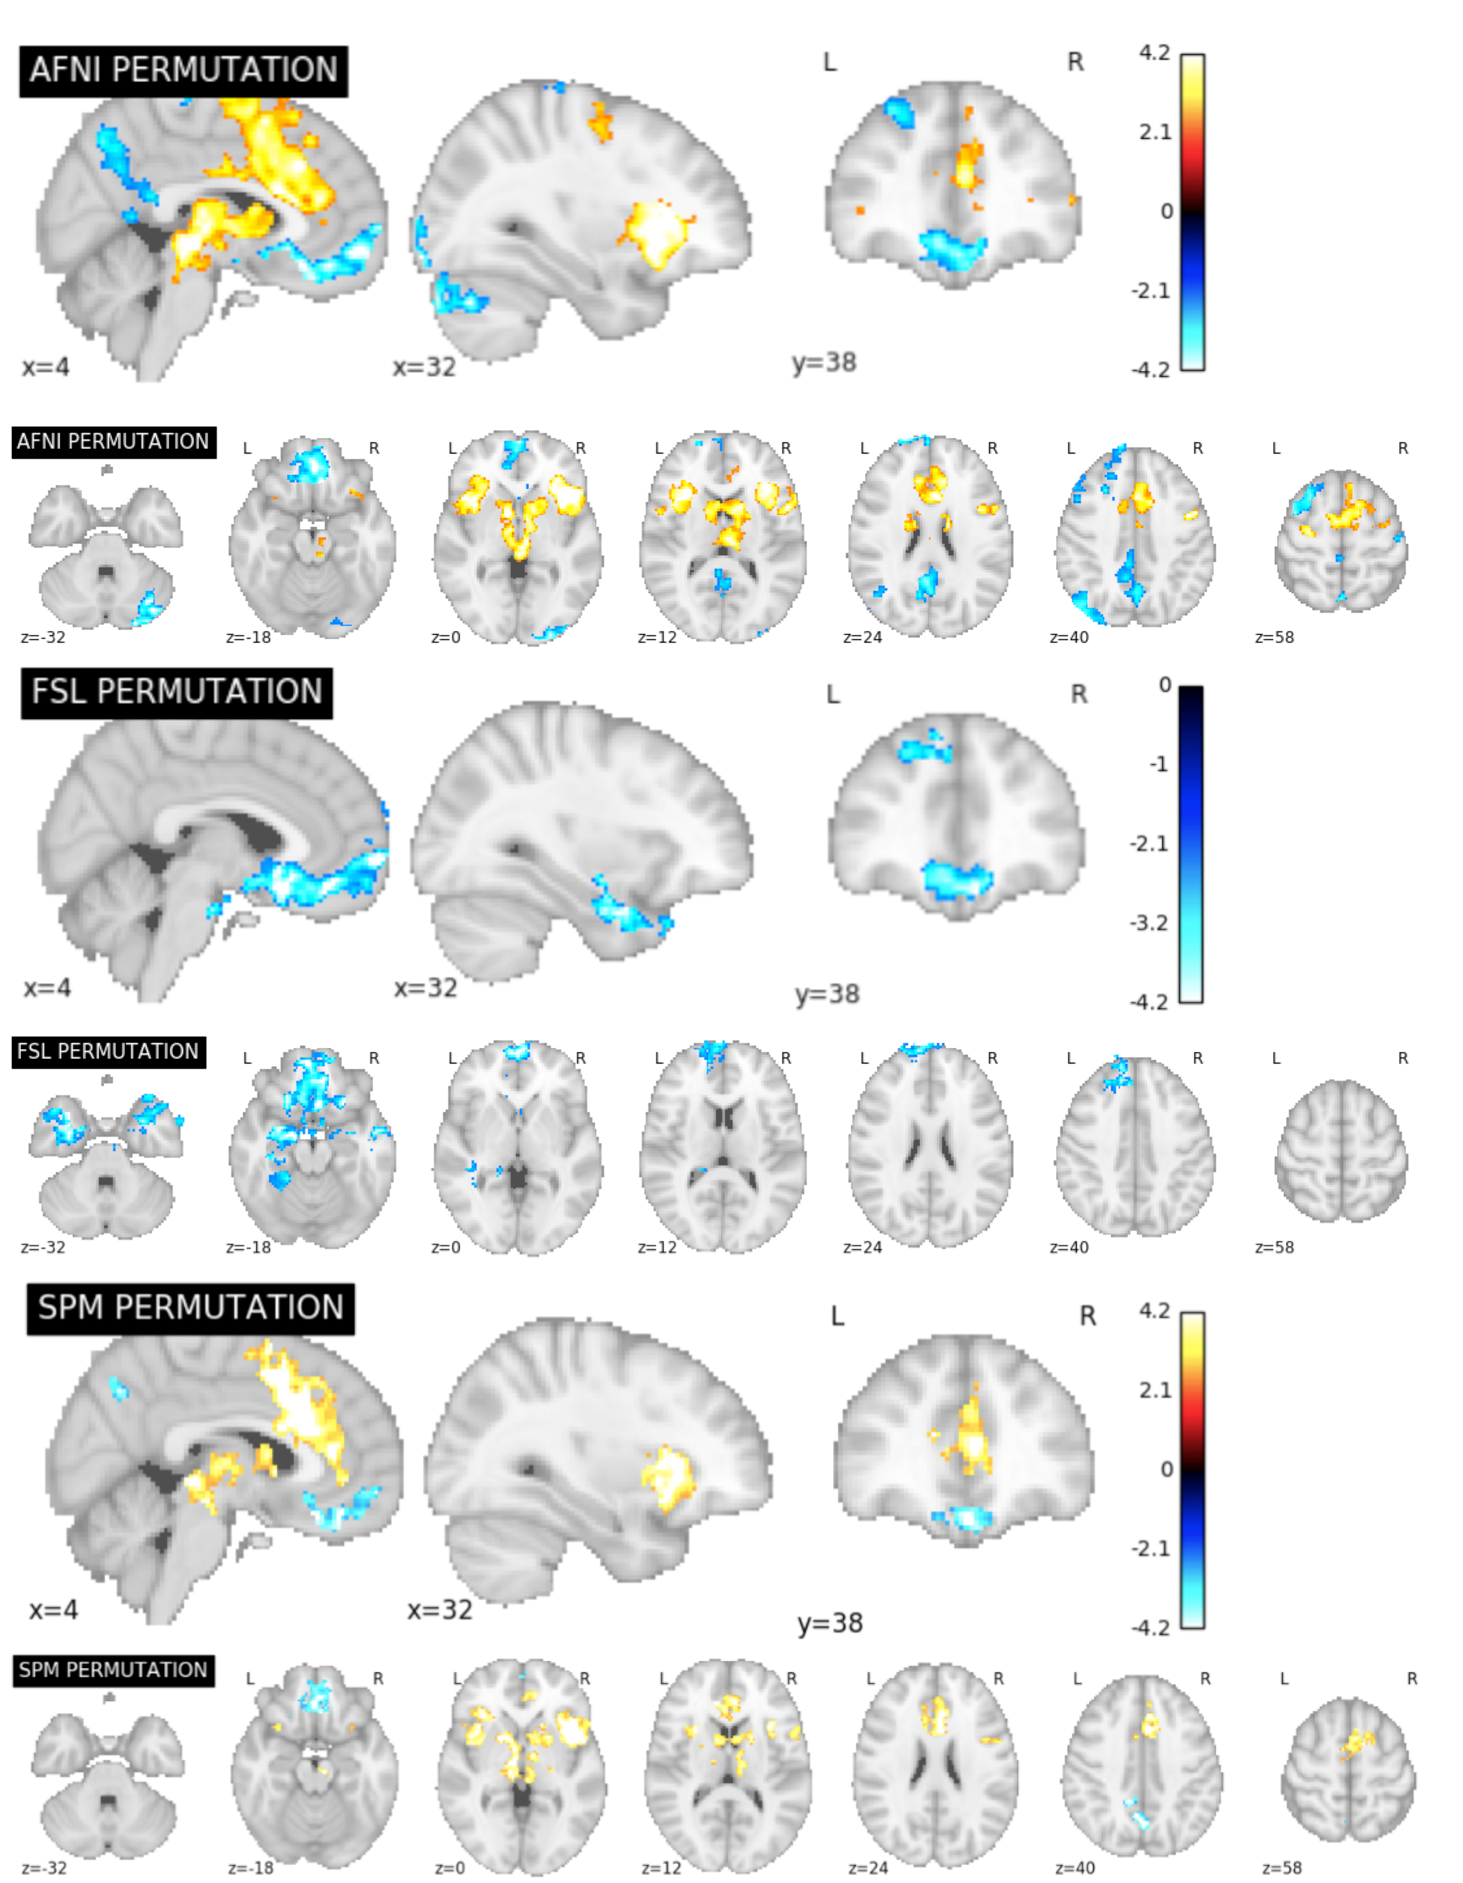
\includegraphics[width=\textwidth]{SC_supp_perm_thresh_ds000001}	
\caption{ds000001 inter-software comparisons, 5\% FWE clusterwise permutation inference}
\label{fig:SC_supp_perm_thresh_ds000001}
\end{figure}

\begin{figure}[htbp]
\centering
	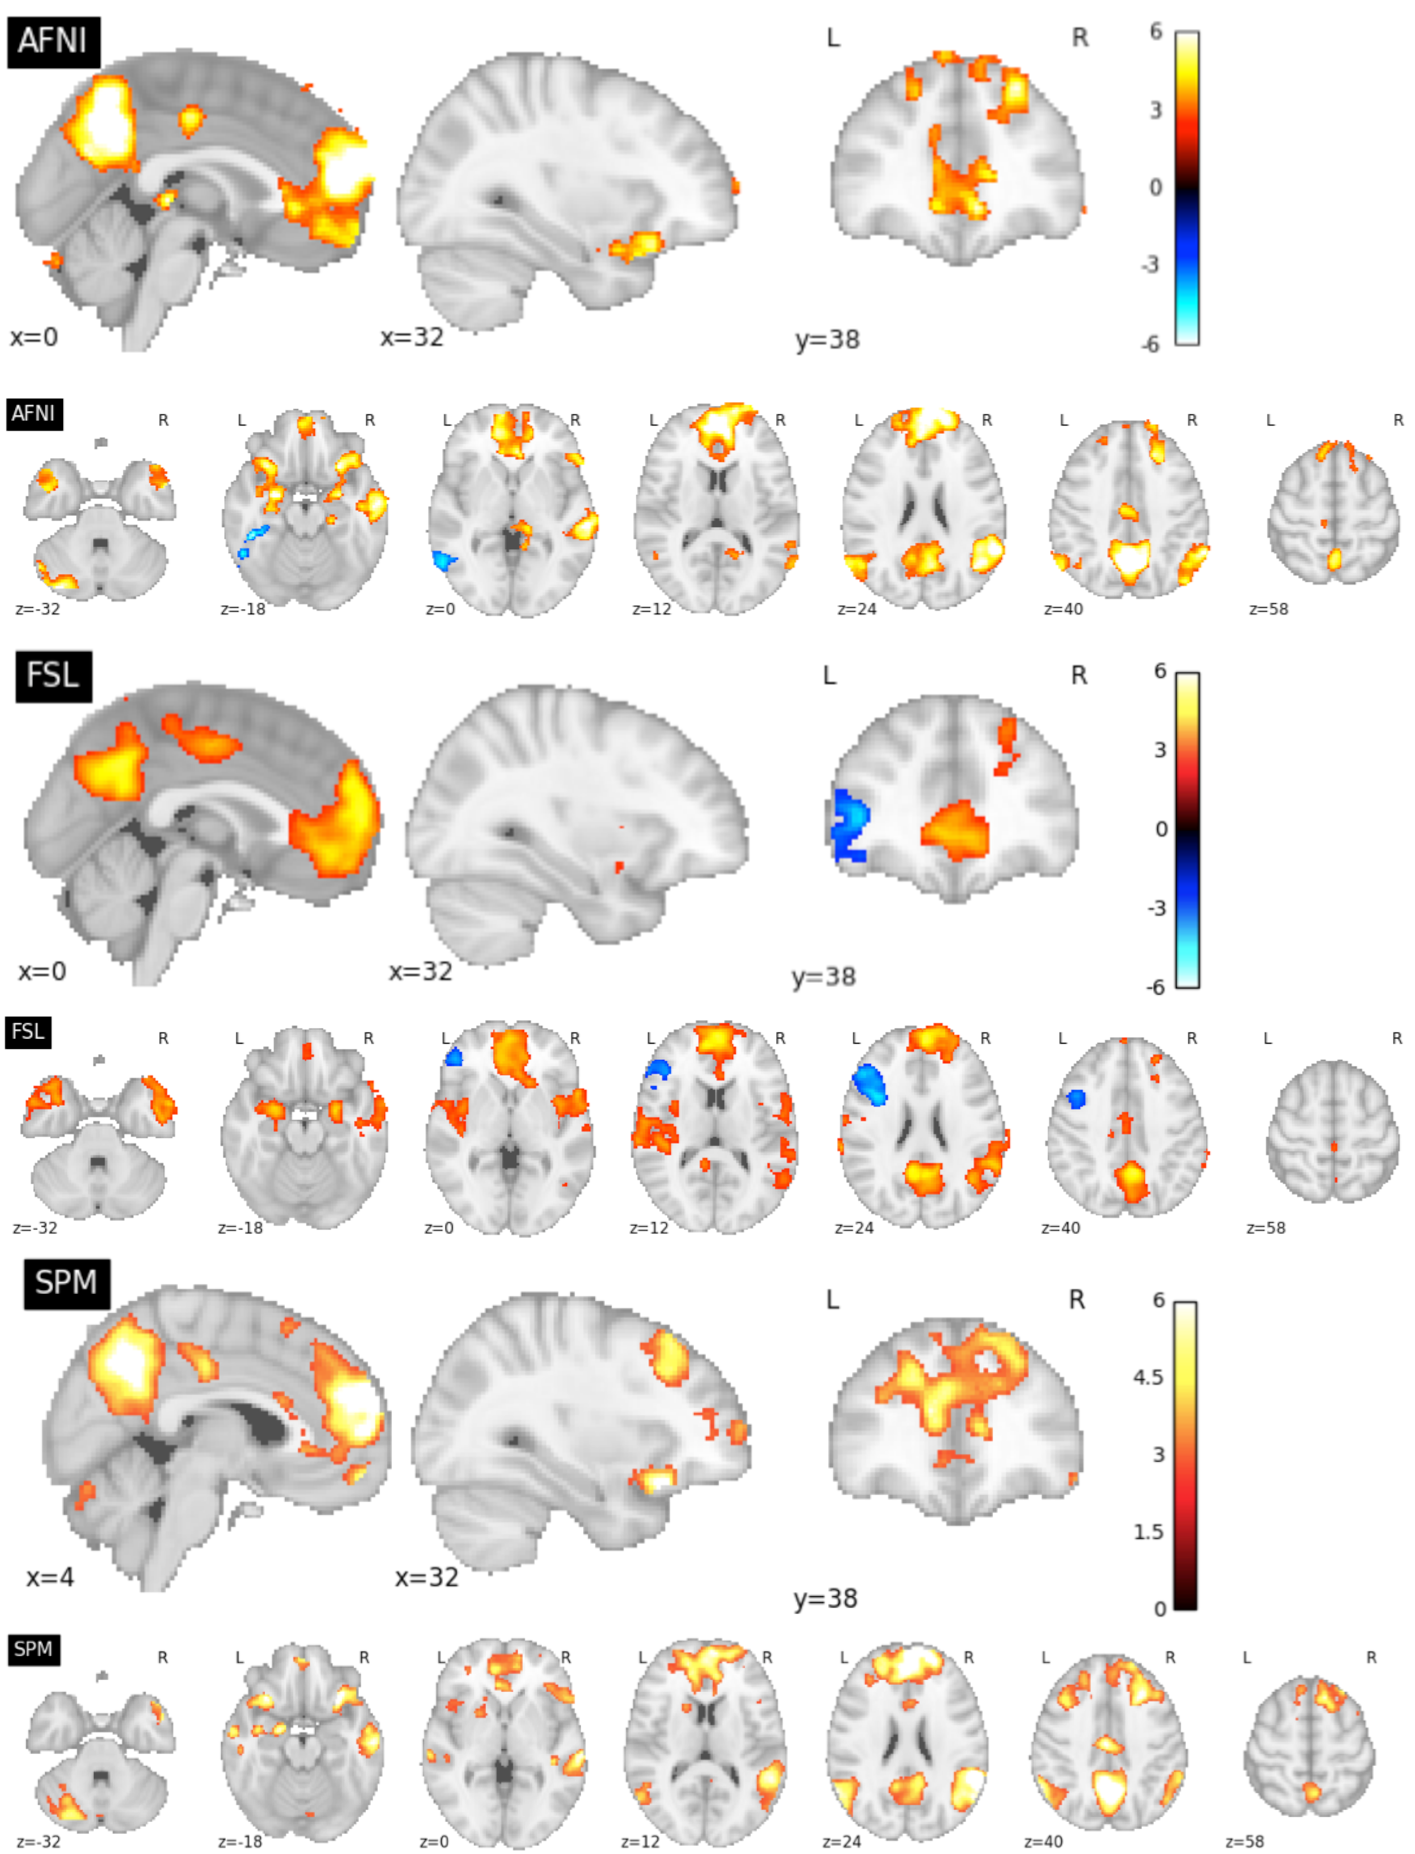
\includegraphics[width=\textwidth]{SC_supp_thresh_ds000109}	
\caption{ds000109 inter-software comparisons, 5\% FWE clusterwise inference}
\label{fig:SC_supp_thresh_ds000109}
\end{figure}

\begin{figure}[htbp]
\centering
	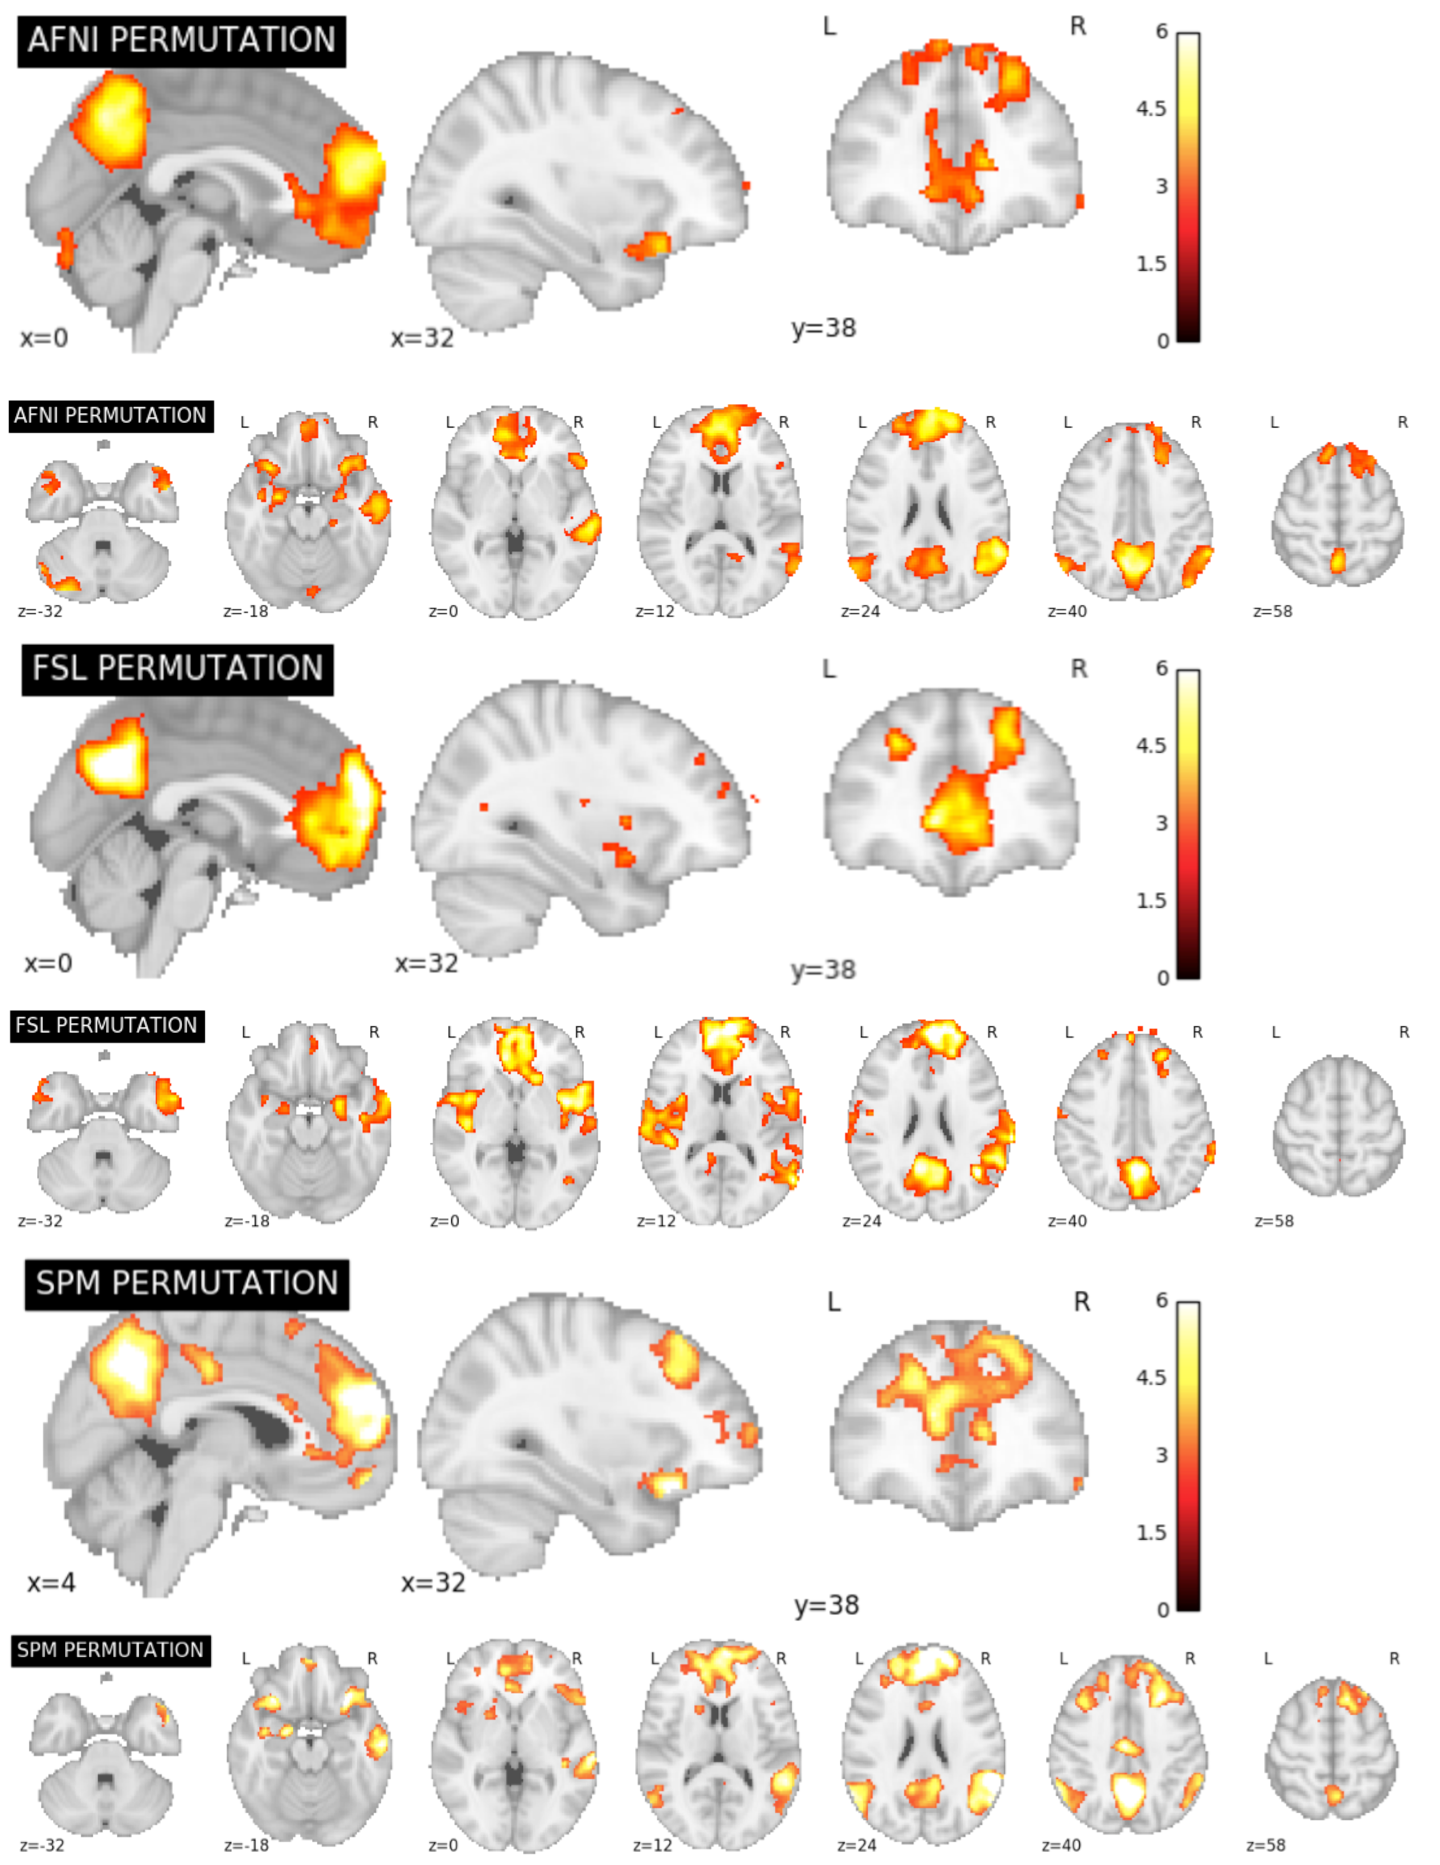
\includegraphics[width=\textwidth]{SC_supp_perm_thresh_ds000109}	
\caption{ds000109 inter-software comparisons, 5\% FWE clusterwise permutation inference}
\label{fig:SC_supp_perm_thresh_ds000109}
\end{figure}

\begin{figure}[htbp]
\centering
	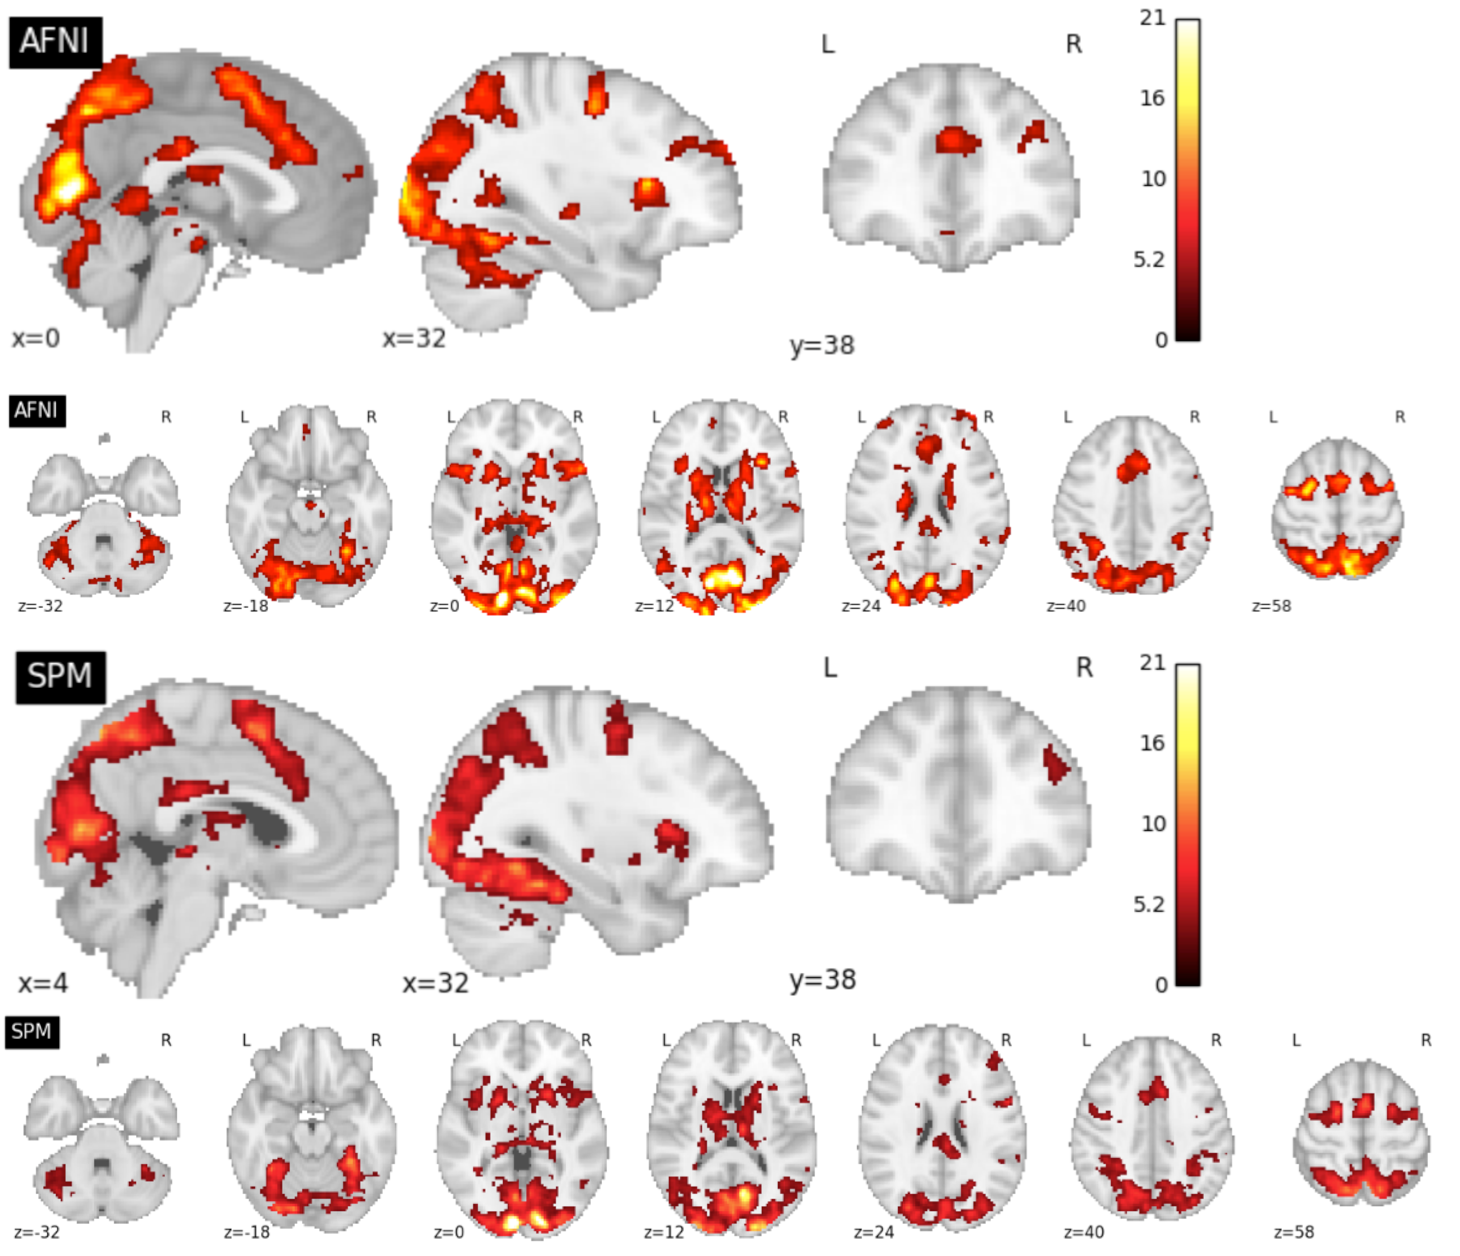
\includegraphics[width=\textwidth]{SC_supp_thresh_ds000120}	
\caption{ds000120 inter-software comparisons, 5\% FWE clusterwise inference}
\label{fig:SC_supp_thresh_ds000120}
\end{figure}

\begin{figure}[htbp]
\centering
	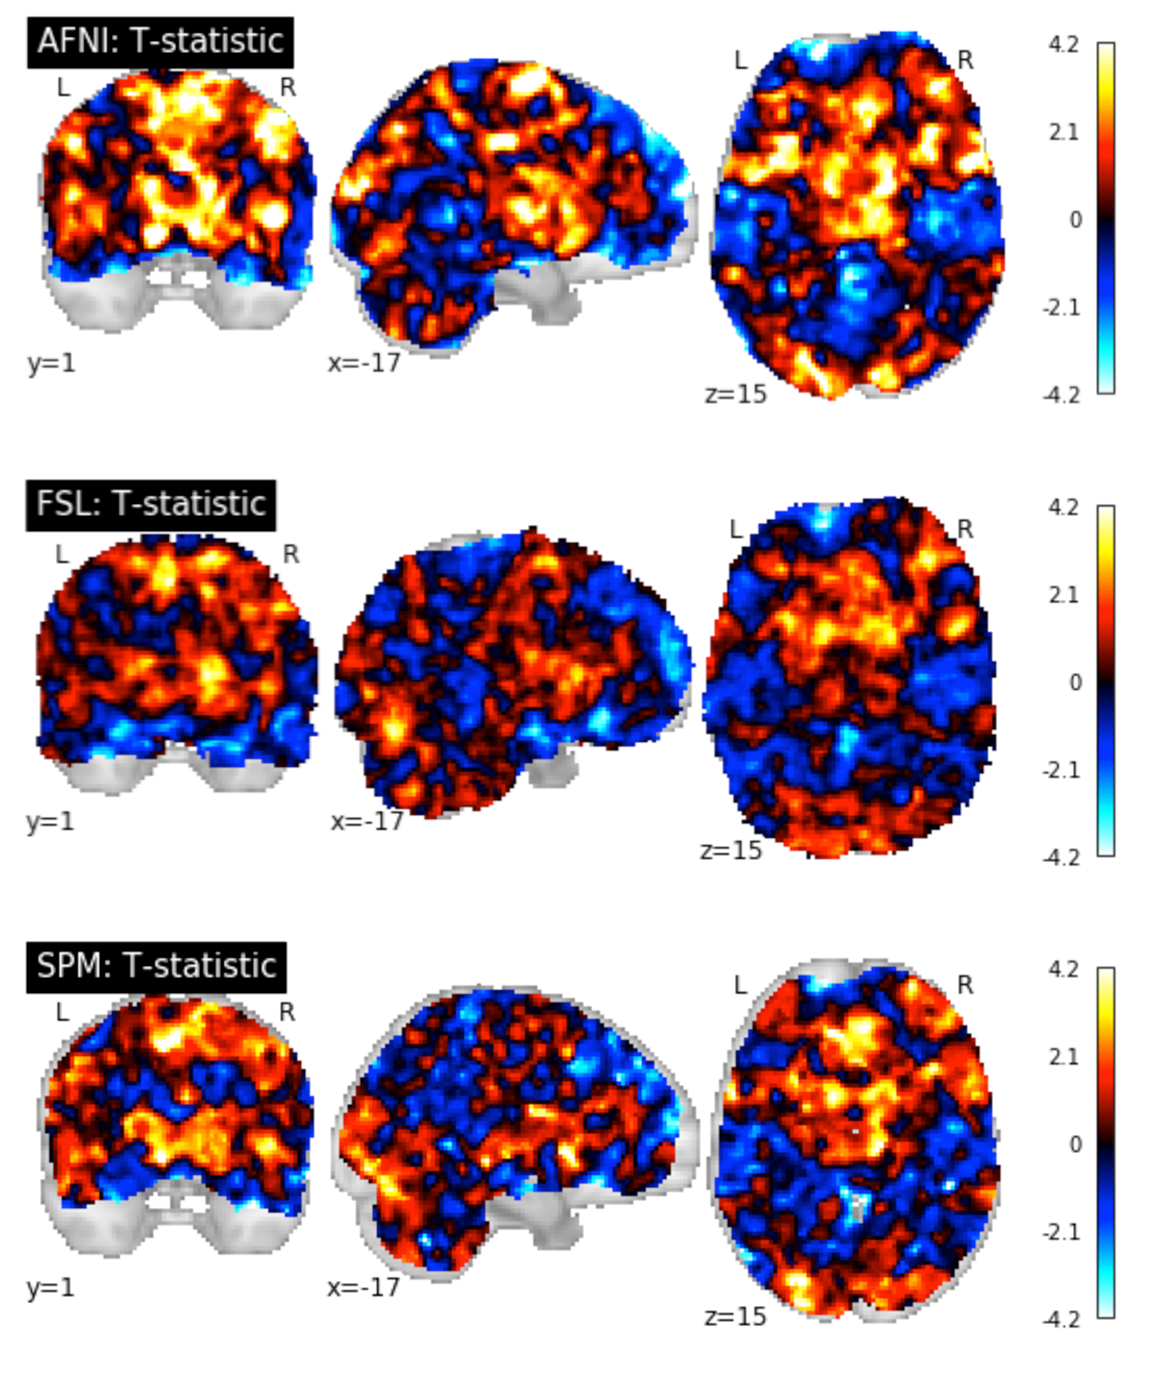
\includegraphics[width=\textwidth]{SC_supp_unthresh_ds000001}	
\caption{ds000001 inter-software comparisons, $t$-statistic maps}
\label{fig:SC_supp_unthresh_ds000001}
\end{figure}

\begin{figure}[htbp]
\centering
	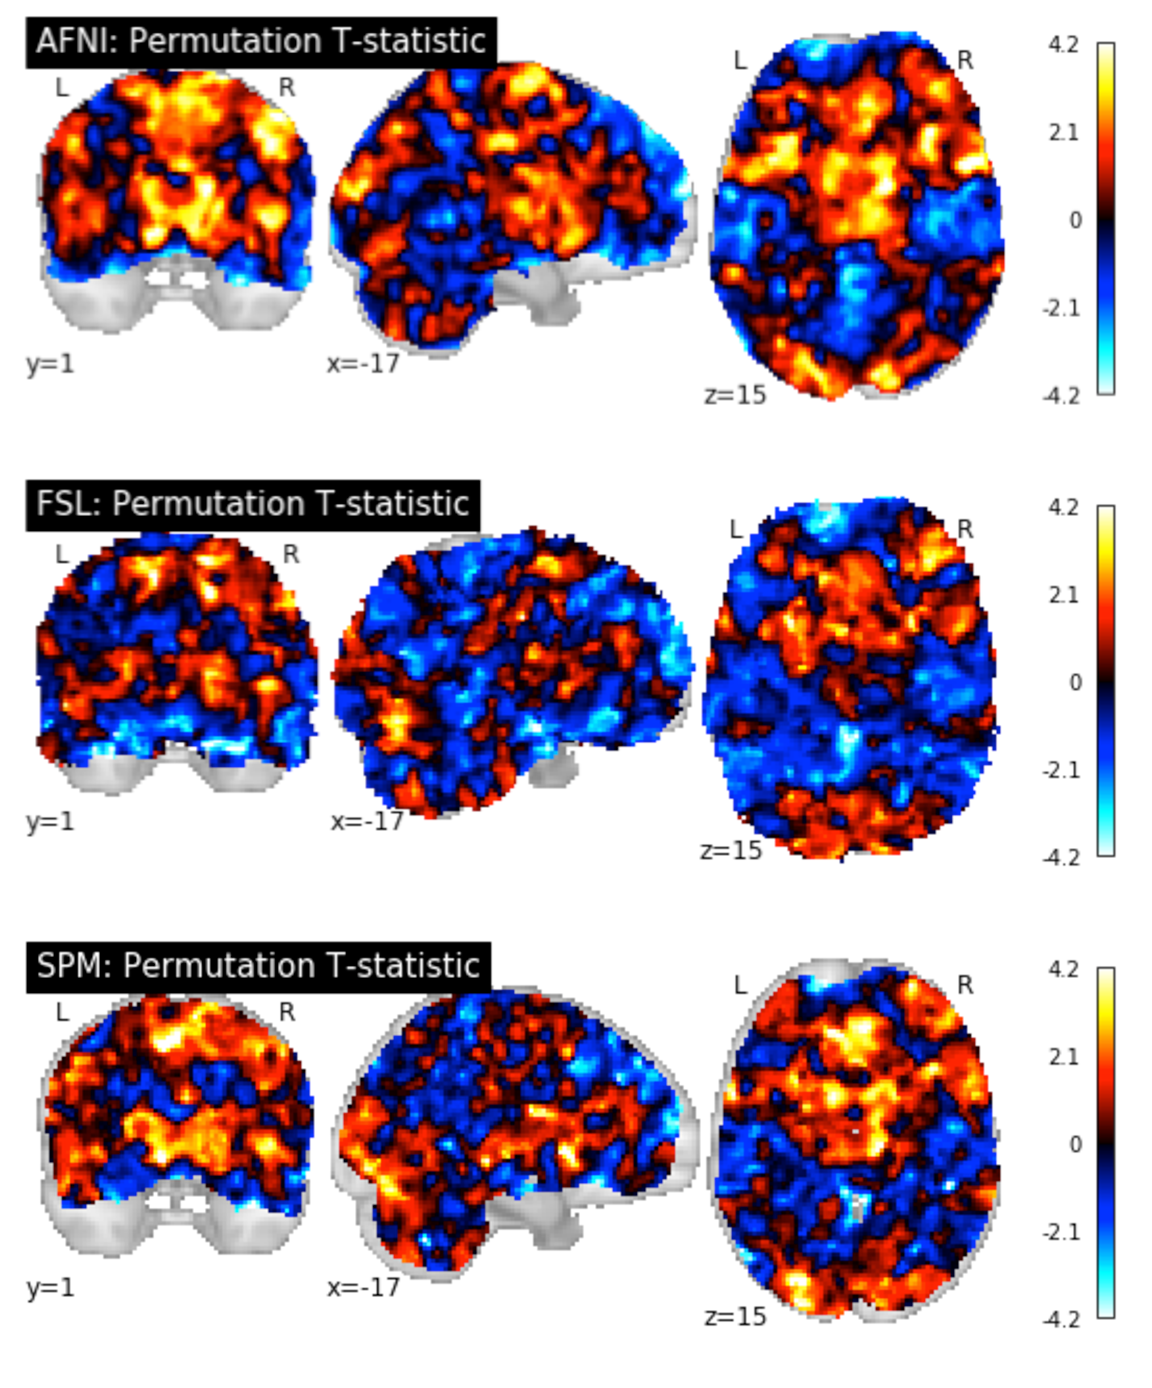
\includegraphics[width=\textwidth]{SC_supp_perm_unthresh_ds000001}	
\caption{ds000001 inter-software comparisons, $t$-statistic maps from permutation}
\label{fig:SC_supp_perm_unthresh_ds000001}
\end{figure}

\begin{figure}[htbp]
\centering
	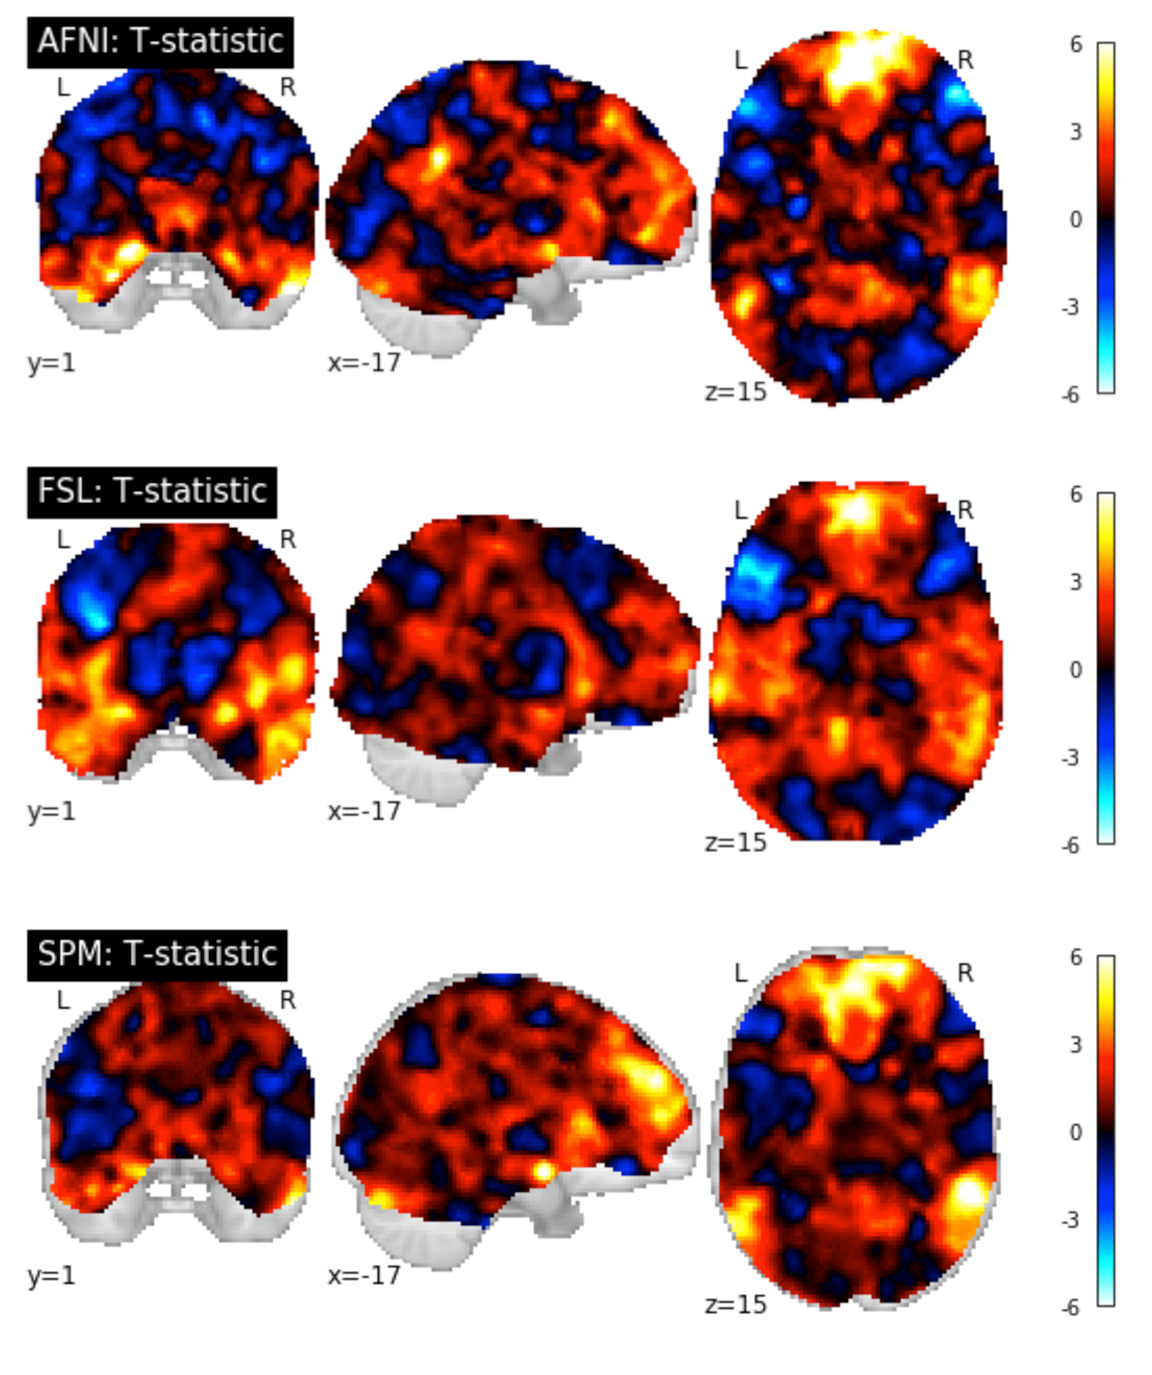
\includegraphics[width=\textwidth]{SC_supp_unthresh_ds000109}	
\caption{ds000109 inter-software comparisons, $t$-statistic maps}
\label{fig:SC_supp_unthresh_ds000109}
\end{figure}

\begin{figure}[htbp]
\centering
	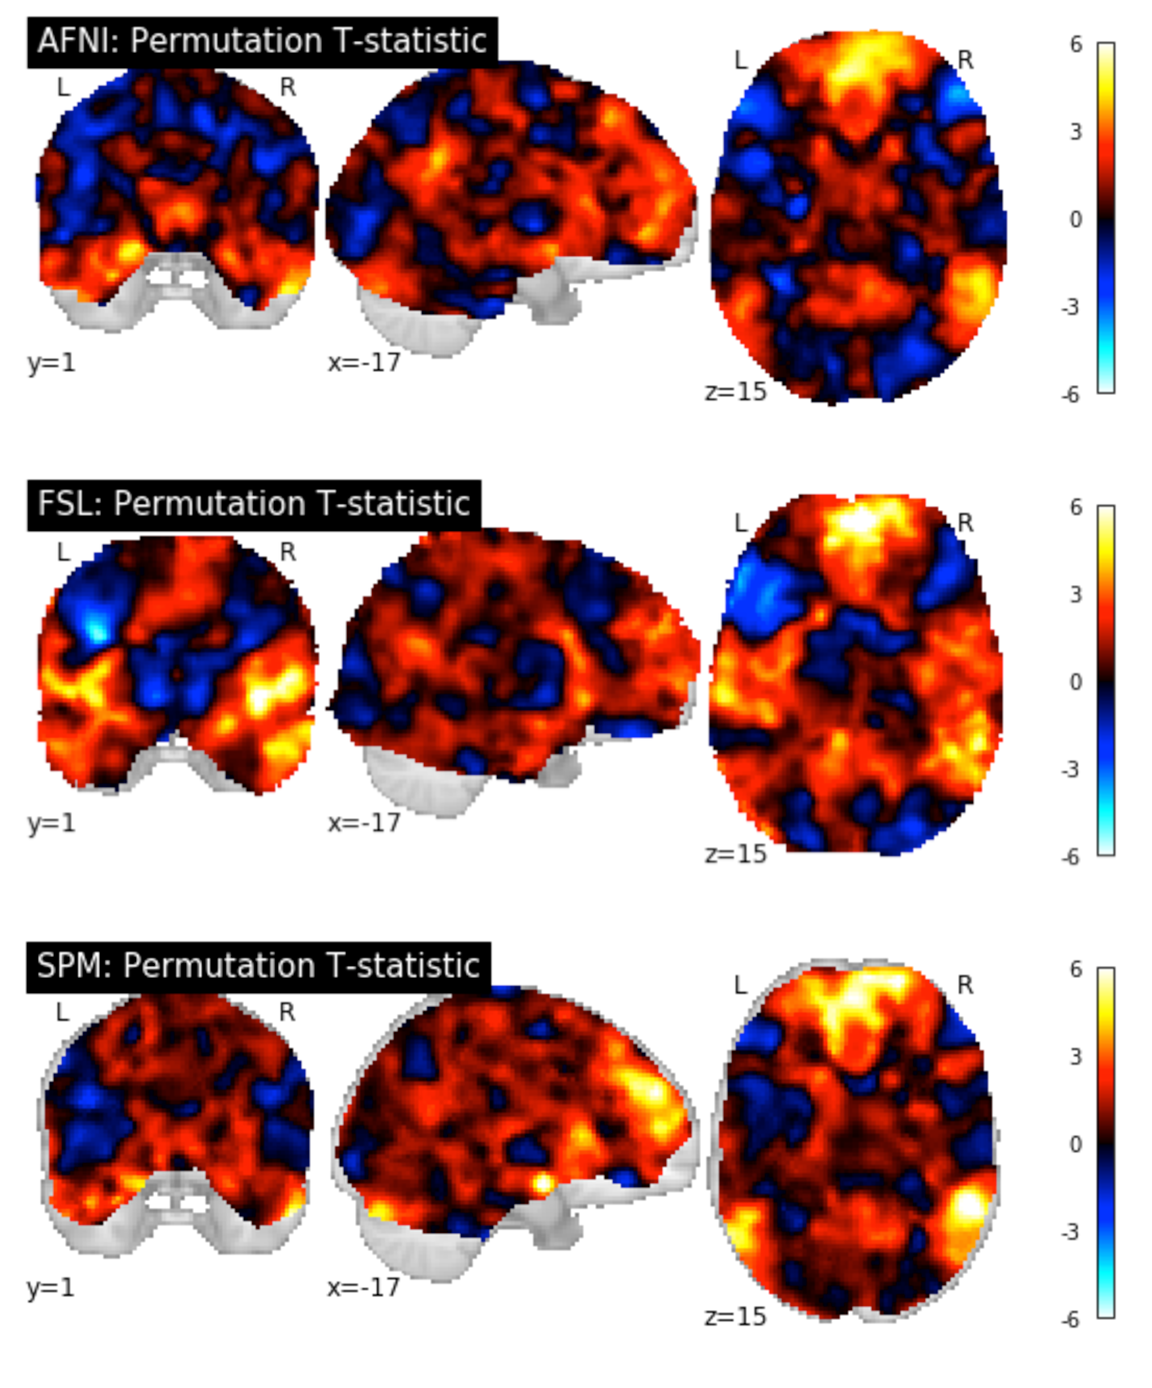
\includegraphics[width=\textwidth]{SC_supp_perm_unthresh_ds000109}	
\caption{ds000109 inter-software comparisons, $t$-statistic maps from permutation}
\label{fig:SC_supp_perm_unthresh_ds000109}
\end{figure}

\begin{figure}[htbp]
\centering
	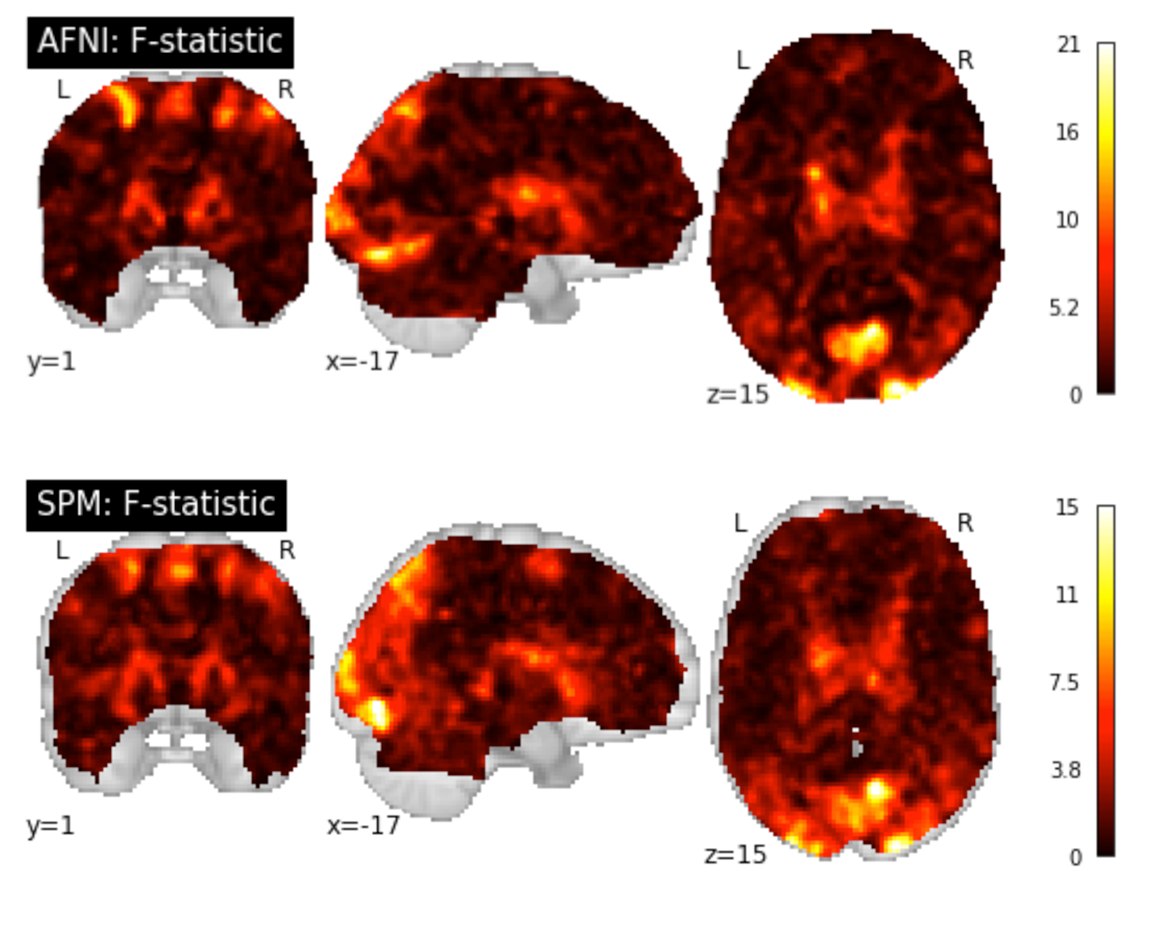
\includegraphics[width=\textwidth]{SC_supp_unthresh_ds000120}	
\caption{ds0001020 inter-software comparisons, $F$-statistic maps}
\label{fig:SC_supp_unthresh_ds000120}
\end{figure}

\begin{figure}[htbp]
\centering
	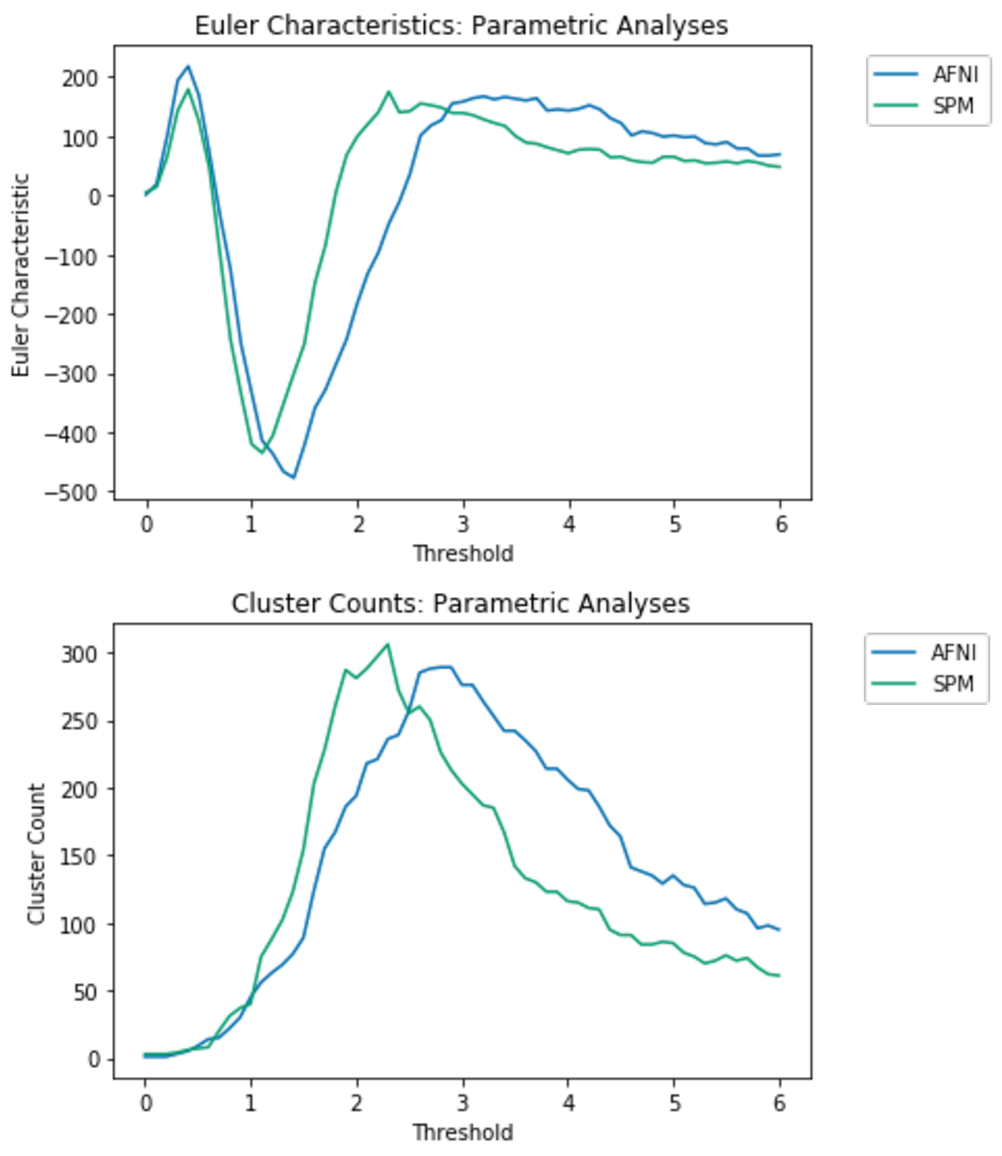
\includegraphics[width=\textwidth]{SC_supp_ECs}	
\caption{ds000120 inter-software comparisons, Euler characeristic and cluster count curves for $F$-statistic maps}
\label{fig:SC_supp_ECs}
\end{figure}

\begin{figure}[htbp]
\centering
	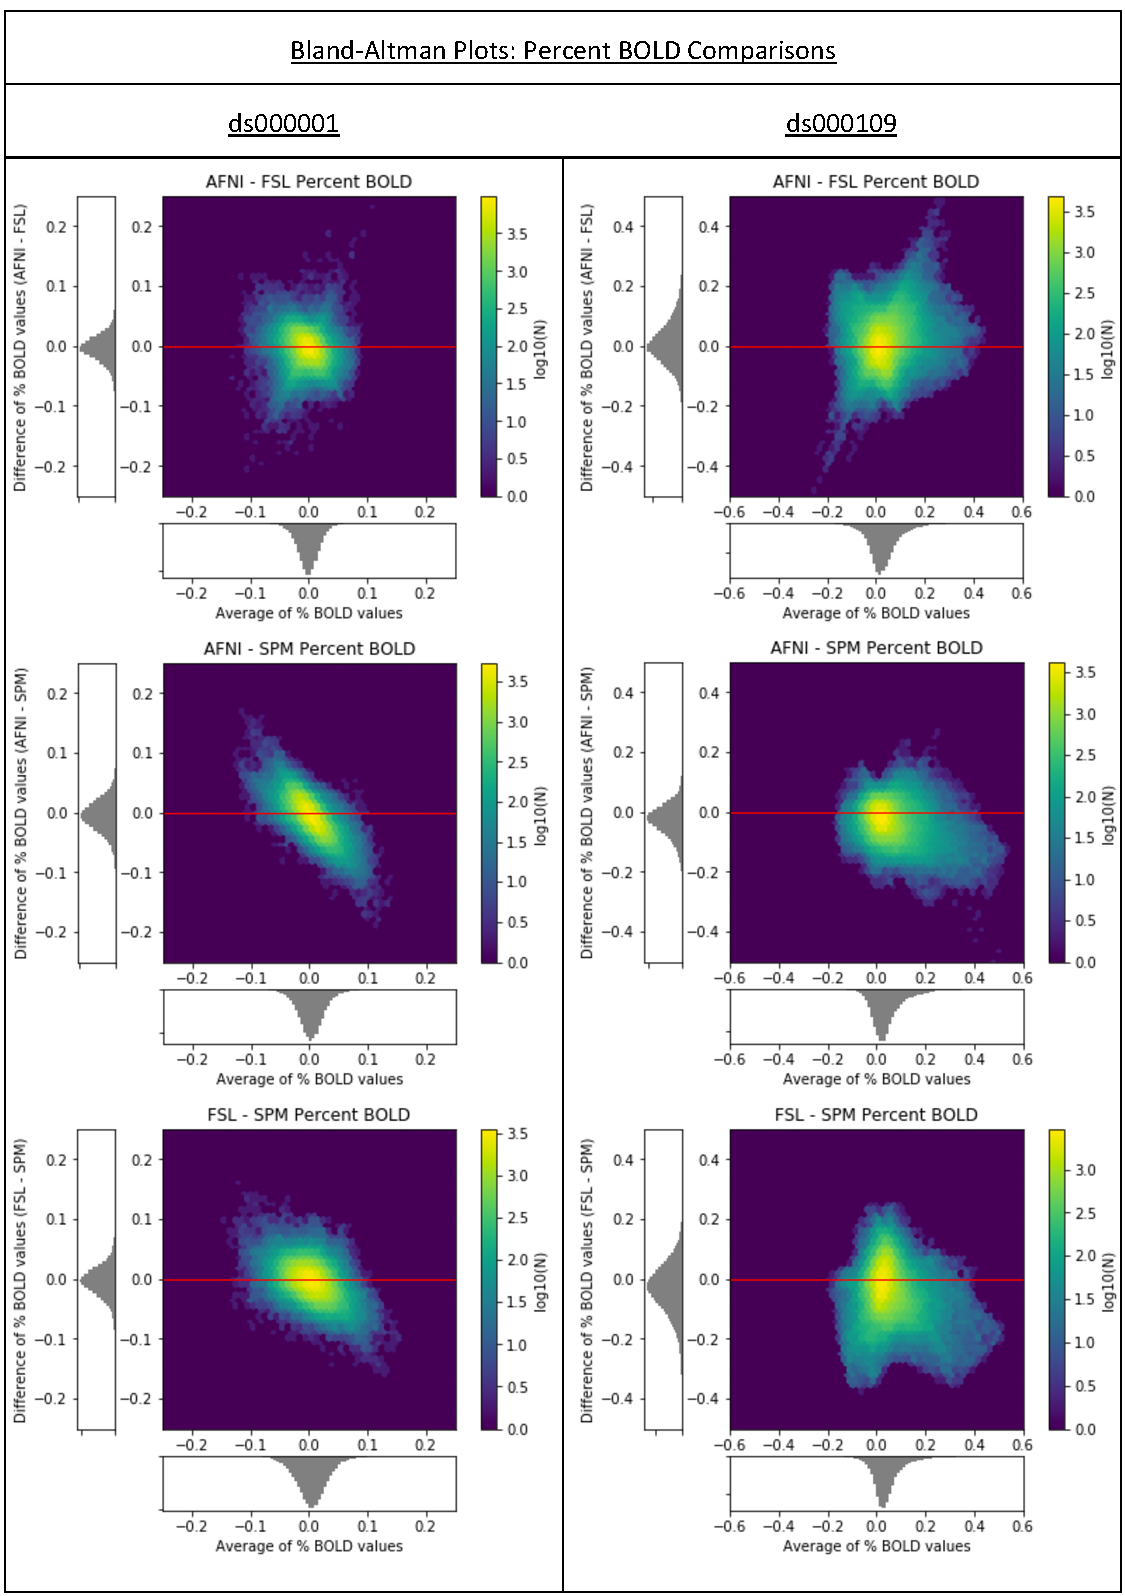
\includegraphics[width=\textwidth]{SC_supp_BOLD_BAs}	
\caption{Bland-Altman percent BOLD comparisons}
\label{fig:SC_supp_BOLD_BAs}
\end{figure}


\begin{figure}[htbp]
\centering
	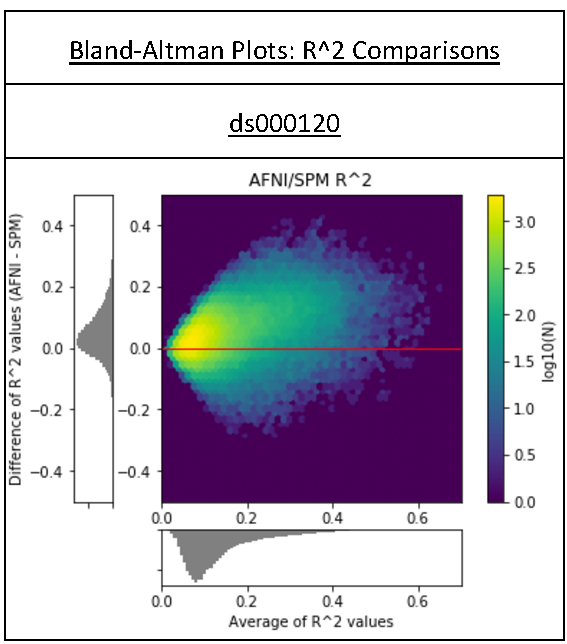
\includegraphics[]{SC_supp_BOLD_BAs_ds000120}	
\caption{ds000120 $R^{2}$ comparisons}
\label{fig:SC_supp_BOLD_BAs_ds000120}
\end{figure}







\chapter{\%BOLD Confidence Sets Supplementary Material}
\section{Supplementary Human Connectome Project Results}
\label{sec:supp_CI_figs}

\begin{table}[htbp]
\hspace*{-0.5cm}
\begin{adjustbox}{center}
\centering
    \begin{tabular}{cm{50mm}m{50mm}m{50mm}}
       \toprule
         Threshold $c$ & \hspace{1.4cm} Sagittal (X = 61) & \ \hspace{1.2cm} Coronal (Y = 75) & \hspace{1.0cm} Axial (Z = 37)\\
        \midrule
        1.0\% BOLD change & 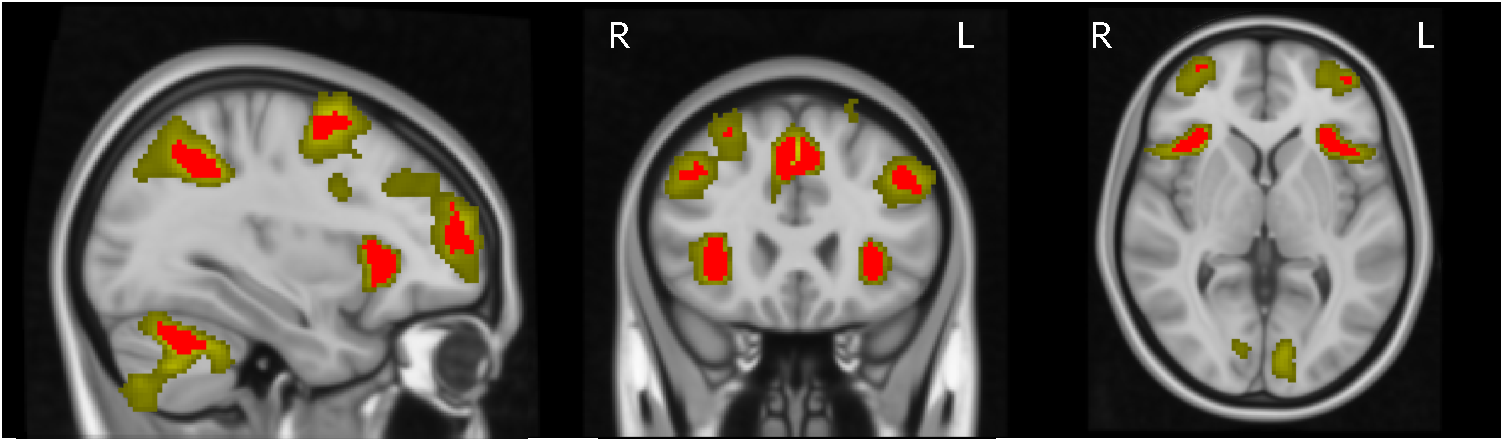
\includegraphics[height=45mm]{CIB_GLM_Fig1_c10.pdf}\\
        1.5\% BOLD change & 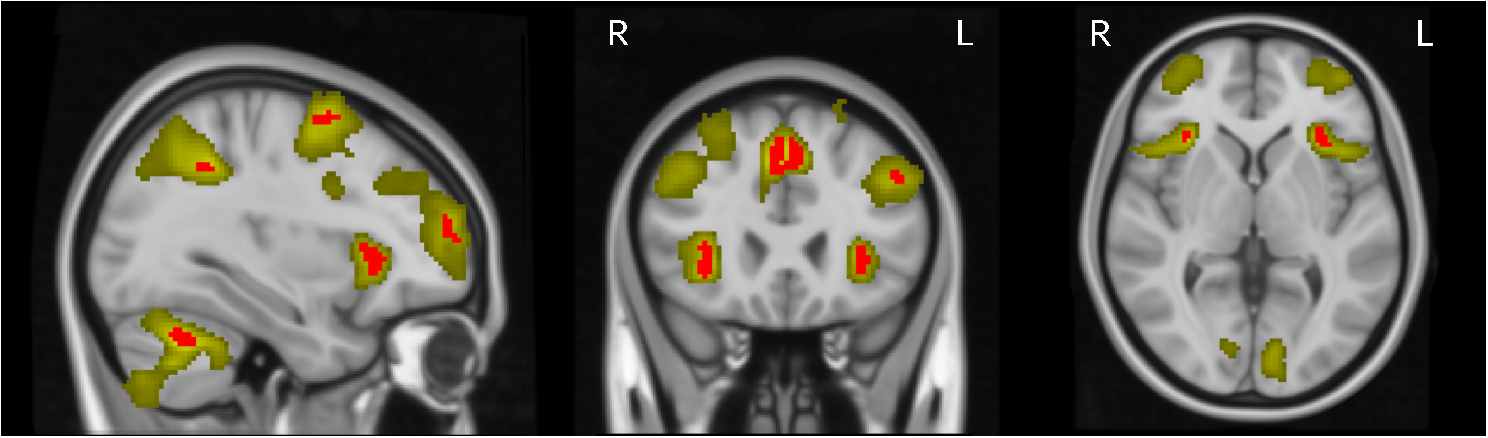
\includegraphics[height=45.5mm]{CIB_GLM_Fig1_c15.pdf}\\
        2.0\% BOLD change & 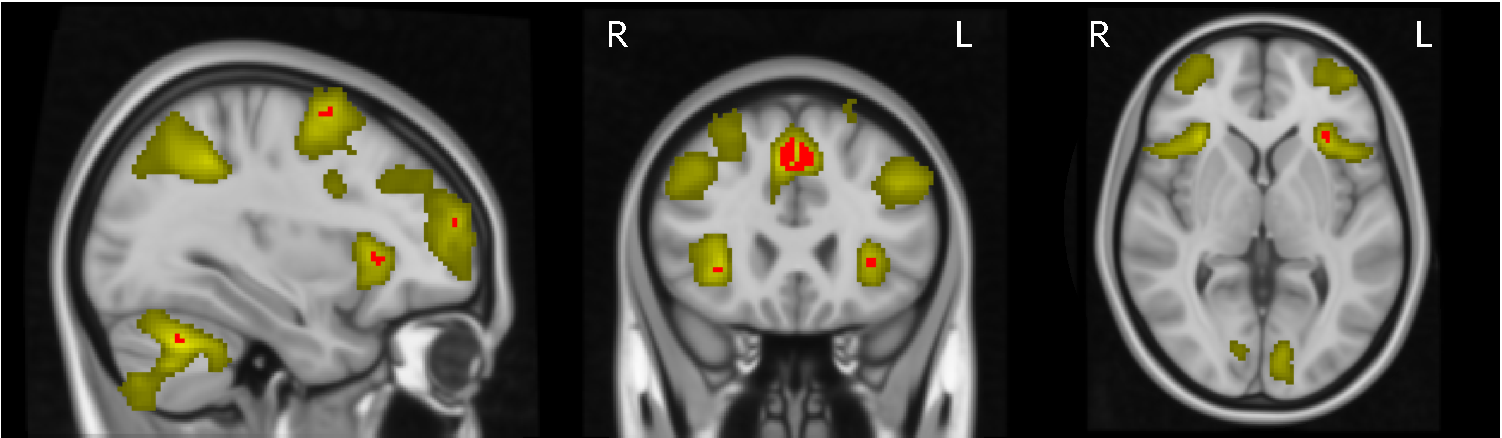
\includegraphics[height=45mm]{CIB_GLM_Fig1_c20.pdf}\\
        \bottomrule
    \end{tabular}
\end{adjustbox}
    \captionof{figure}{Comparing the upper Confidences Sets for the HCP working memory task data (same slice views as Fig. \ref{tbl:HCP_results_one}) with the thresholded $t$-statistic results obtained by applying a traditional group-level one-sample $t$-test, voxelwise $p < 0.05$ FWE correction (green-yellow voxels). While over 25,000 voxels were determined as statistically significant with the standard inference method, less than 5,000 voxels were asserted to have at least a 1.0\% BOLD change by the CSs. In particular, the two statistically significant clusters spanning the left and right side of the frontal lobe contained almost no voxels with a practical effect size of over 1.5\% BOLD change.}
    \label{tbl:Supp_HCP_results_one}
\end{table}

\begin{table}[htbp]
\hspace*{-0.5cm}
\begin{adjustbox}{center}
\centering
    \begin{tabular}{cm{50mm}m{50mm}m{50mm}}
       \toprule
         Threshold $c$ & \hspace{1.4cm} Sagittal (X = 47) & \ \hspace{1.2cm} Coronal (Y = 71) & \hspace{1.0cm} Axial (Z = 60)\\
        \midrule
        1.0\% BOLD change & 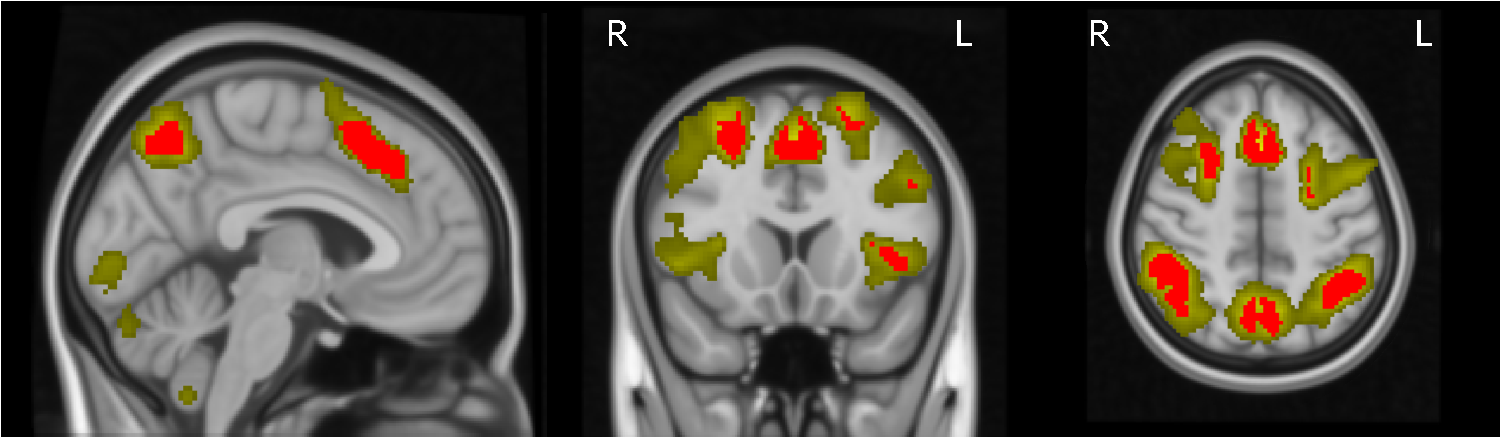
\includegraphics[height=45mm]{CIB_GLM_Fig2_c10.pdf}\\
        1.5\% BOLD change & 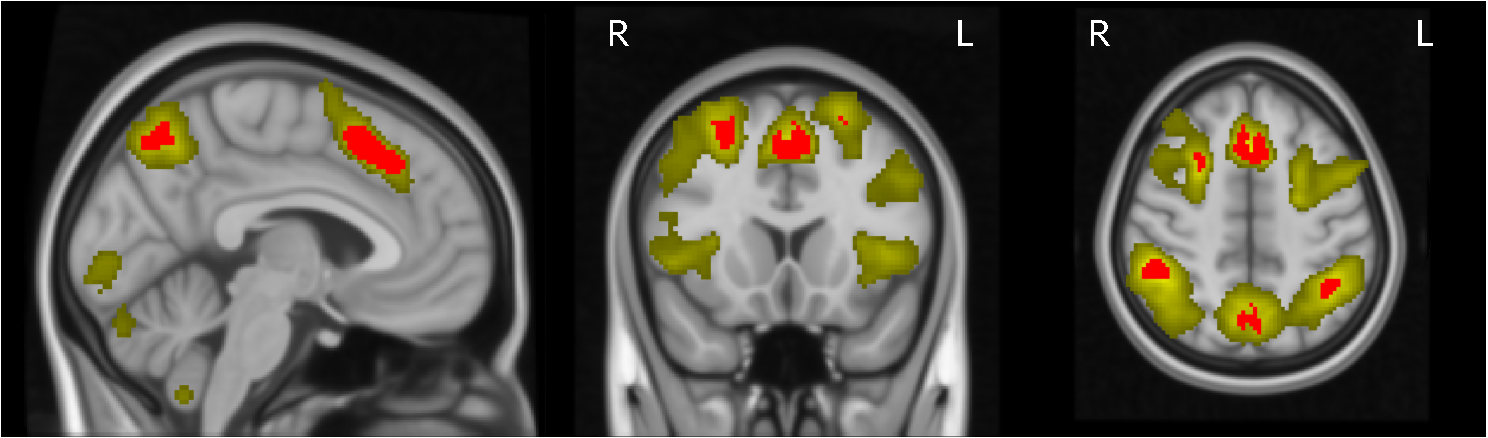
\includegraphics[height=45.5mm]{CIB_GLM_Fig2_c15.pdf}\\
        2.0\% BOLD change & 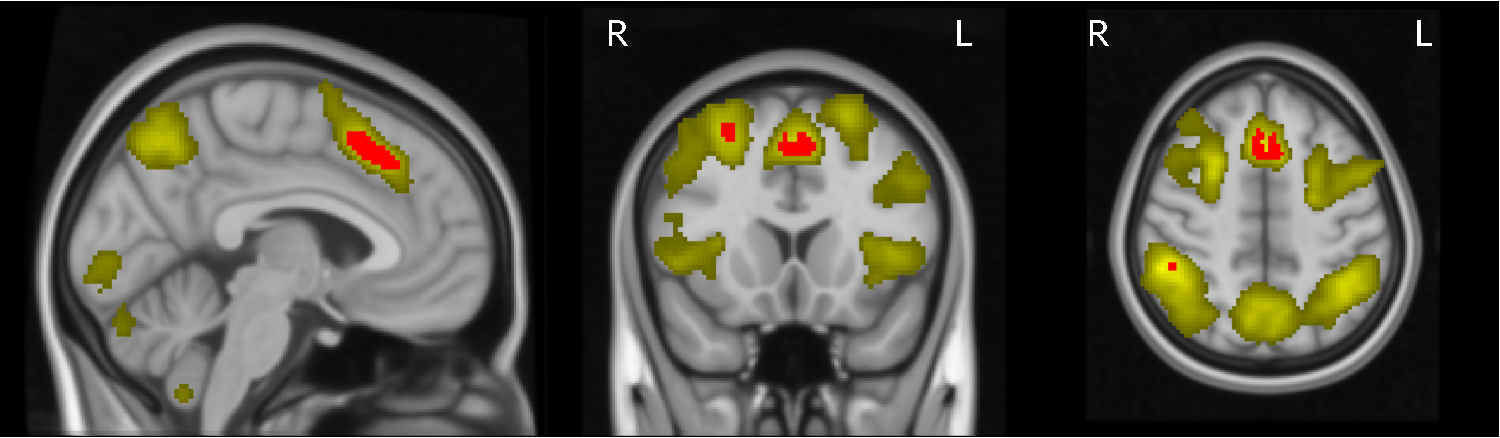
\includegraphics[height=45mm]{CIB_GLM_Fig2_c20.pdf}\\
        \bottomrule
    \end{tabular}
\end{adjustbox}
    \captionof{figure}{Comparing the upper Confidences Sets for the HCP working memory task data (same slice views as Fig. \ref{tbl:HCP_results_two}) with the thresholded $t$-statistic results obtained by applying a traditional group-level one-sample $t$-test, voxelwise $p < 0.05$ FWE correction (green-yellow voxels). While one large statistically significant cluster covers the supramarginal gyrus, angular gyrus and precuneous, the CSs localize the precise areas with practically significant effect sizes within each of these regions.}
    \label{tbl:Supp_HCP_results_two}
\end{table}

\section{Supplementary Tables}
\label{sec:supp_CI_tabs}
\begin{onehalfspace}
\begin{table}[htbp]
\vspace{-5.0em}
\caption{Empirical coverage results for the 2D simulations using nominal (nom.) coverage levels $1-\alpha = 80\%, 90\%$ and $95\%$. Results are shown for applying the Wild $t$-Bootstrap method to the residual field along the estimated boundary $\dAhatc$ (top) and the true boundary $\dAc$ (bottom).}
\centering
\hspace*{-1.5cm}
\begin{tabular}{@{}p{0.14\textwidth}*{4}{L{\dimexpr0.26\textwidth-2\tabcolsep\relax}}@{}}
\toprule
& \multicolumn{2}{c}{\textbf{2D Signal 1. (Ramp)}} &
\multicolumn{2}{c}{\textbf{2D Signal 2. (Circle)}} \\
\cmidrule(r{4pt}){2-3} \cmidrule(l){4-5}
& \textbf{Standard Dev 1.} & \ \textbf{Standard Dev 2.} & \ \ \textbf{Standard Dev 1.} & \ \textbf{Standard Dev 2.}\\
\midrule
$\mathbf{\dAhatc}$  \\[-0.4em]
$80\%$ nom.  \\[-0.4em]
$N = \hphantom{1}60$ & 90.13\% $\pm$ 0.54\% & 87.57\% $\pm$ 0.60\% & 78.13\% $\pm$ 0.75\% & 80.23\% $\pm$ 0.73\% \\[-0.4em]
$\hphantom{N{}={}}120$ & 87.53\% $\pm$ 0.60\% & 88.40\% $\pm$ 0.58\% & 80.53\% $\pm$ 0.72\% & 78.70\% $\pm$ 0.75\% \\[-0.4em]
$\hphantom{N{}={}}240$ & 87.43\% $\pm$ 0.61\% & 87.33\% $\pm$ 0.61\% & 79.73\% $\pm$ 0.73\% & 79.53\% $\pm$ 0.74\% \\[-0.4em]
$\hphantom{N{}={}}480$ & 87.40\% $\pm$ 0.61\% & 85.07\% $\pm$ 0.65\% & 78.50\% $\pm$ 0.75\% & 77.40\% $\pm$ 0.76\%\\
$90\%$ nom.  \\[-0.4em]
$N = \hphantom{1}60$ & 95.53\% $\pm$ 0.38\% & 94.83\% $\pm$ 0.40\% & 88.90\% $\pm$ 0.57\% & 89.90\% $\pm$ 0.55\% \\[-0.4em]
$\hphantom{N{}={}}120$ & 94.07\% $\pm$ 0.43\% & 93.73\% $\pm$ 0.44\% & 90.13\% $\pm$ 0.54\% & 89.40\% $\pm$ 0.56\% \\[-0.4em]
$\hphantom{N{}={}}240$ & 94.23\% $\pm$ 0.43\% & 93.60\% $\pm$ 0.45\% & 89.17\% $\pm$ 0.57\% & 90.17\% $\pm$ 0.54\% \\[-0.4em]
$\hphantom{N{}={}}480$ & 93.50\% $\pm$ 0.45\% & 93.33\% $\pm$ 0.46\% & 89.30\% $\pm$ 0.56\% & 88.40\% $\pm$ 0.58\%\\ 
$95\%$ nom.  \\[-0.4em]
$N = \hphantom{1}60$ & 97.67\% $\pm$ 0.28\% & 97.33\% $\pm$ 0.29\% & 94.10\% $\pm$ 0.43\% & 94.60\% $\pm$ 0.41\% \\[-0.4em]
$\hphantom{N{}={}}120$ & 97.13\% $\pm$ 0.30\% & 96.60\% $\pm$ 0.33\% & 94.40\% $\pm$ 0.42\% & 94.37\% $\pm$ 0.42\% \\[-0.4em]
$\hphantom{N{}={}}240$ & 97.30\% $\pm$ 0.30\% & 97.07\% $\pm$ 0.31\% & 94.43\% $\pm$ 0.42\% & 95.53\% $\pm$ 0.38\% \\[-0.4em]
$\hphantom{N{}={}}480$ & 96.97\% $\pm$ 0.31\% & 97.13\% $\pm$ 0.30\% & 94.80\% $\pm$ 0.41\% & 93.73\% $\pm$ 0.44\%\\
\midrule
$\mathbf{\dAc}$\\[-0.4em]
$80\%$ nom.\\[-0.4em]
$N = \hphantom{1}60$ & 60.27\% $\pm$ 0.89\% & 57.30\% $\pm$ 0.90\% & 78.17\% $\pm$ 0.75\% & 80.23\% $\pm$ 0.73\% \\[-0.4em]
$\hphantom{N{}={}}120$ & 66.03\% $\pm$ 0.86\% & 68.30\% $\pm$ 0.85\% & 80.53\% $\pm$ 0.72\% & 78.67\% $\pm$ 0.75\%\\[-0.4em]
$\hphantom{N{}={}}240$ & 71.10\% $\pm$ 0.83\% & 72.23\% $\pm$ 0.82\% & 79.83\% $\pm$ 0.73\% & 79.57\% $\pm$ 0.74\% \\[-0.4em]
$\hphantom{N{}={}}480$ & 76.27\% $\pm$ 0.78\% & 76.17\% $\pm$ 0.78\% & 78.57\% $\pm$ 0.75\% & 77.40\% $\pm$ 0.76\%\\ 
$90\%$ nom.  \\[-0.4em]
$N = \hphantom{1}60$ & 78.47\% $\pm$ 0.75\% & 76.60\% $\pm$ 0.77\% & 88.97\% $\pm$ 0.57\% & 90.00\% $\pm$ 0.55\% \\[-0.4em]
$\hphantom{N{}={}}120$ & 81.67\% $\pm$ 0.71\% & 83.40\% $\pm$ 0.68\% & 90.20\% $\pm$ 0.54\% & 89.43\% $\pm$ 0.56\% \\[-0.4em]
$\hphantom{N{}={}}240$ & 85.20\% $\pm$ 0.65\% & 85.83\% $\pm$ 0.64\% & 89.17\% $\pm$ 0.57\% & 90.17\% $\pm$ 0.54\% \\[-0.4em]
$\hphantom{N{}={}}480$ & 88.50\% $\pm$ 0.58\% & 87.23\% $\pm$ 0.61\% & 89.27\% $\pm$ 0.57\% & 88.43\% $\pm$ 0.58\%\\ 
$95\%$ nom.  \\[-0.4em]
$N = \hphantom{1}60$ & 88.97\% $\pm$ 0.57\% & 87.27\% $\pm$ 0.61\% & 94.17\% $\pm$ 0.43\% & 94.57\% $\pm$ 0.41\% \\[-0.4em]
$\hphantom{N{}={}}120$ & 89.87\% $\pm$ 0.55\% & 90.67\% $\pm$ 0.53\% & 94.47\% $\pm$ 0.42\% & 94.30\% $\pm$ 0.42\% \\[-0.4em]
$\hphantom{N{}={}}240$ & 92.07\% $\pm$ 0.49\% & 92.47\% $\pm$ 0.48\% & 94.40\% $\pm$ 0.42\% & 95.50\% $\pm$ 0.39\% \\[-0.4em]
$\hphantom{N{}={}}480$ & 94.23\% $\pm$ 0.43\% & 94.10\% $\pm$ 0.43 \% & 94.87\% $\pm$ 0.40\% & 93.73\% $\pm$ 0.44\%\\
\bottomrule
\end{tabular}
\label{tbl:supp_CI_2D_results}
\end{table}

\pagebreak

\begin{table}[htbp]
\vspace{-5.0em}
\caption{Empirical coverage results for the 3D simulations using nominal (nom.) coverage levels $1-\alpha = 80\%, 90\%$ and $95\%$. Results are shown for applying the Wild $t$-Bootstrap method to the residual field along the estimated boundary $\dAhatc$ (top) and the true boundary $\dAc$ (bottom).}
\centering
\hspace*{-1.5cm}
\begin{tabular}{@{}p{0.14\textwidth}*{4}{L{\dimexpr0.26\textwidth-2\tabcolsep\relax}}@{}}
\toprule
& \multicolumn{2}{c}{\textbf{3D Signal 1. (Small Sphere)}} &
\multicolumn{2}{c}{\textbf{3D Signal 2. (Large Sphere)}} \\
\cmidrule(r{4pt}){2-3} \cmidrule(l){4-5}
& \textbf{Standard Dev 1.} & \ \textbf{Standard Dev 2.} & \ \ \textbf{Standard Dev 1.} & \ \textbf{Standard Dev 2.}\\
\midrule
$\mathbf{\dAhatc}$  \\[-0.4em]
$80\%$ nom.  \\[-0.4em]
$N = \hphantom{1}60$ & 83.40\% $\pm$ 0.68\% & 83.77\% $\pm$ 0.67\% & 85.10\% $\pm$ 0.65\% & 85.73\% $\pm$ 0.64\% \\[-0.4em]
$\hphantom{N{}={}}120$ & 83.67\% $\pm$ 0.67\% & 84.03\% $\pm$ 0.67\% & 85.87\% $\pm$ 0.64\% & 85.23\% $\pm$ 0.65\% \\[-0.4em]
$\hphantom{N{}={}}240$ & 84.03\% $\pm$ 0.67\% & 83.77\% $\pm$ 0.67\% & 85.23\% $\pm$ 0.65\% & 85.40\% $\pm$ 0.64\% \\[-0.4em]
$\hphantom{N{}={}}480$ & 85.03\% $\pm$ 0.65\% & 82.20\% $\pm$ 0.70\% & 87.67\% $\pm$ 0.60\% & 85.30\% $\pm$ 0.65\%\\
$90\%$ nom.  \\[-0.4em]
$N = \hphantom{1}60$ & 92.30\% $\pm$ 0.49\% & 92.87\% $\pm$ 0.47\% & 92.40\% $\pm$ 0.48\% & 93.47\% $\pm$ 0.45\% \\[-0.4em]
$\hphantom{N{}={}}120$ & 92.07\% $\pm$ 0.49\% & 91.27\% $\pm$ 0.52\% & 93.00\% $\pm$ 0.47\% & 93.50\% $\pm$ 0.45\% \\[-0.4em]
$\hphantom{N{}={}}240$ & 92.33\% $\pm$ 0.49\% & 92.87\% $\pm$ 0.47\% & 93.30\% $\pm$ 0.46\% & 92.90\% $\pm$ 0.47\% \\[-0.4em]
$\hphantom{N{}={}}480$ & 93.03\% $\pm$ 0.46\% & 91.53\% $\pm$ 0.51\% & 93.50\% $\pm$ 0.45\% & 93.47\% $\pm$ 0.45\%\\ 
$95\%$ nom.  \\[-0.4em]
$N = \hphantom{1}60$ & 96.87\% $\pm$ 0.32\% & 96.83\% $\pm$ 0.32\% & 96.40\% $\pm$ 0.34\% & 96.70\% $\pm$ 0.33\% \\[-0.4em]
$\hphantom{N{}={}}120$ & 96.07\% $\pm$ 0.35\% & 95.60\% $\pm$ 0.37\% & 96.97\% $\pm$ 0.31\% & 97.10\% $\pm$ 0.31\% \\[-0.4em]
$\hphantom{N{}={}}240$ & 96.20\% $\pm$ 0.35\% & 96.83\% $\pm$ 0.32\% & 96.23\% $\pm$ 0.35\% & 96.90\% $\pm$ 0.32\% \\[-0.4em]
$\hphantom{N{}={}}480$ & 96.30\% $\pm$ 0.34\% & 96.13\% $\pm$ 0.35\% & 96.83\% $\pm$ 0.32\% & 93.80\% $\pm$ 0.44\%\\
\midrule
$\mathbf{\dAc}$\\[-0.4em]
$80\%$ nom.\\[-0.4em]
$N = \hphantom{1}60$ & 83.60\% $\pm$ 0.68\% & 83.90\% $\pm$ 0.67\% & 85.20\% $\pm$ 0.65\% & 85.80\% $\pm$ 0.64\% \\[-0.4em]
$\hphantom{N{}={}}120$ & 83.80\% $\pm$ 0.67\% & 83.93\% $\pm$ 0.67\% & 85.90\% $\pm$ 0.64\% & 85.23\% $\pm$ 0.65\%\\[-0.4em]
$\hphantom{N{}={}}240$ & 84.03\% $\pm$ 0.67\% & 83.90\% $\pm$ 0.67\% & 85.27\% $\pm$ 0.65\% & 85.40\% $\pm$ 0.64\% \\[-0.4em]
$\hphantom{N{}={}}480$ & 85.03\% $\pm$ 0.65\% & 82.27\% $\pm$ 0.70\% & 87.73\% $\pm$ 0.60\% & 85.37\% $\pm$ 0.65\%\\ 
$90\%$ nom.  \\[-0.4em]
$N = \hphantom{1}60$ & 92.43\% $\pm$ 0.48\% & 92.90\% $\pm$ 0.47\% & 92.37\% $\pm$ 0.48\% & 93.40\% $\pm$ 0.45\% \\[-0.4em]
$\hphantom{N{}={}}120$ & 91.97\% $\pm$ 0.50\% & 91.43\% $\pm$ 0.51\% & 92.97\% $\pm$ 0.47\% & 93.60\% $\pm$ 0.45\% \\[-0.4em]
$\hphantom{N{}={}}240$ & 92.37\% $\pm$ 0.48\% & 92.90\% $\pm$ 0.47\% & 93.33\% $\pm$ 0.46\% & 92.90\% $\pm$ 0.47\% \\[-0.4em]
$\hphantom{N{}={}}480$ & 93.03\% $\pm$ 0.46\% & 91.40\% $\pm$ 0.51\% & 93.57\% $\pm$ 0.45\% & 93.47\% $\pm$ 045\%\\ 
$95\%$ nom.  \\[-0.4em]
$N = \hphantom{1}60$ & 96.87\% $\pm$ 0.32\% & 96.93\% $\pm$ 0.31\% & 96.37\% $\pm$ 0.34\% & 96.70\% $\pm$ 0.33\% \\[-0.4em]
$\hphantom{N{}={}}120$ & 96.07\% $\pm$ 0.35\% & 95.53\% $\pm$ 0.38\% & 96.97\% $\pm$ 0.31\% & 97.13\% $\pm$ 0.30\% \\[-0.4em]
$\hphantom{N{}={}}240$ & 96.17\% $\pm$ 0.35\% & 96.93\% $\pm$ 0.31\% & 96.23\% $\pm$ 0.35\% & 96.80\% $\pm$ 0.32\% \\[-0.4em]
$\hphantom{N{}={}}480$ & 96.33\% $\pm$ 0.34\% & 96.13\% $\pm$ 0.35\% & 96.77\% $\pm$ 0.32\% & 96.80\% $\pm$ 0.32\% \\
\bottomrule
\end{tabular}
\label{tbl:supp_CI_3D_results}
\end{table}

\begin{table}[htbp]
\vspace{-5.0em}
\caption*{\textbf{Table 2. (continued)}}
\centering
\hspace*{-1.5cm}
\begin{tabular}{@{}p{0.14\textwidth}*{4}{L{\dimexpr0.26\textwidth-2\tabcolsep\relax}}@{}}
\toprule
& \multicolumn{2}{c}{\textbf{3D Signal 3. (Multiple Spheres)}} &
\multicolumn{2}{c}{\textbf{3D Signal 4. (UK Biobank)}} \\
\cmidrule(r{4pt}){2-3} \cmidrule(l){4-5}
& \textbf{Standard Dev 1.} & \ \textbf{Standard Dev 2.} & \textbf{UK Biobank SD} \\
\midrule
$\mathbf{\dAhatc}$  \\[-0.4em]
$80\%$ nom.  \\[-0.4em]
$N = \hphantom{1}60$ & 89.47\% $\pm$ 0.56\% & 89.20\% $\pm$ 0.57\% & 89.17\% $\pm$ 0.57\% &  \\[-0.4em]
$\hphantom{N{}={}}120$ & 87.60\% $\pm$ 0.60\% & 88.17\% $\pm$ 0.59\% & 87.17\% $\pm$ 0.61\% & \\[-0.4em]
$\hphantom{N{}={}}240$ & 86.17\% $\pm$ 0.63\% & 86.33\% $\pm$ 0.63\% & 86.27\% $\pm$ 0.63\% & \\[-0.4em]
$\hphantom{N{}={}}480$ & 86.13\% $\pm$ 0.63\% & 86.10\% $\pm$ 0.63\% & 87.67\% $\pm$ 0.60\%\\ 
$90\%$ nom.  \\[-0.4em]
$N = \hphantom{1}60$ & 95.20\% $\pm$ 0.39\% & 94.87\% $\pm$ 0.40\% & 95.23\% $\pm$ 0.39\% & \\[-0.4em]
$\hphantom{N{}={}}120$ & 94.53\% $\pm$ 0.42\% & 93.97\% $\pm$ 0.43\% & 94.63\% $\pm$ 0.41\% & \\[-0.4em]
$\hphantom{N{}={}}240$ & 93.67\% $\pm$ 0.44\% & 93.17\% $\pm$ 0.46\% & 93.73\% $\pm$ 0.44\% & \\[-0.4em]
$\hphantom{N{}={}}480$ & 93.97\% $\pm$ 0.43\% & 93.87\% $\pm$ 0.44\% & 93.50\% $\pm$ 0.45\%\\ 
$95\%$ nom.  \\[-0.4em]
$N = \hphantom{1}60$ & 97.93\% $\pm$ 0.26\% & 97.73\% $\pm$ 0.27\% & 97.37\% $\pm$ 0.29\% & \\[-0.4em]
$\hphantom{N{}={}}120$ & 97.37\% $\pm$ 0.29\% & 97.47\% $\pm$ 0.29\% & 97.73\% $\pm$ 0.27\% & \\[-0.4em]
$\hphantom{N{}={}}240$ & 97.23\% $\pm$ 0.30\% & 96.50\% $\pm$ 0.34\% & 96.93\% $\pm$ 0.31\% & \\[-0.4em]
$\hphantom{N{}={}}480$ & 97.23\% $\pm$ 0.30\% & 97.63\% $\pm$ 0.28\% & 96.83\% $\pm$ 0.32\%\\
\midrule
$\mathbf{\dAc}$\\[-0.4em]
$80\%$ nom.\\[-0.4em]
$N = \hphantom{1}60$ & 84.30\% $\pm$ 0.66\% & 85.33\% $\pm$ 0.65\% & 83.30\% $\pm$ 0.68\% & \\[-0.4em]
$\hphantom{N{}={}}120$ & 84.93\% $\pm$ 0.65\% & 86.20\% $\pm$ 0.63\% & 85.13\% $\pm$ 0.65\% & \\[-0.4em]
$\hphantom{N{}={}}240$ & 85.73\% $\pm$ 0.64\% & 85.60\% $\pm$ 0.64\% & 84.97\% $\pm$ 0.65\% & \\[-0.4em]
$\hphantom{N{}={}}480$ & 86.03\% $\pm$ 0.63\% & 85.97\% $\pm$ 0.63\% & 87.73\% $\pm$ 0.60\%\\ 
$90\%$ nom.  \\[-0.4em]
$N = \hphantom{1}60$ & 92.93\% $\pm$ 0.47\% & 92.20\% $\pm$ 0.49\% & 92.77\% $\pm$ 0.47\% & \\[-0.4em]
$\hphantom{N{}={}}120$ & 93.20\% $\pm$ 0.46\% & 93.27\% $\pm$ 0.46\% & 93.50\% $\pm$ 0.45\% & \\[-0.4em]
$\hphantom{N{}={}}240$ & 93.37\% $\pm$ 0.45\% & 93.07\% $\pm$ 0.46\% & 92.67\% $\pm$ 0.48\% & \\[-0.4em]
$\hphantom{N{}={}}480$ & 93.97\% $\pm$ 0.43\% & 93.80\% $\pm$ 0.44\% & 93.57\% $\pm$ 0.45\%\\ 
$95\%$ nom.  \\[-0.4em]
$N = \hphantom{1}60$ & 96.80\% $\pm$ 0.32\% & 96.50\% $\pm$ 0.34\% & 96.70\% $\pm$ 0.33\% & \\[-0.4em]
$\hphantom{N{}={}}120$ & 96.90\% $\pm$ 0.32\% & 96.83\% $\pm$ 0.32\% & 97.07\% $\pm$ 0.31\% & \\[-0.4em]
$\hphantom{N{}={}}240$ & 97.20\% $\pm$ 0.30\% & 96.30\% $\pm$ 0.34\% & 96.40\% $\pm$ 0.34\% & \\[-0.4em]
$\hphantom{N{}={}}480$ & 97.27\% $\pm$ 0.30\% & 97.63\% $\pm$ 0.28\% & 96.77\% $\pm$ 0.32\%\\
\bottomrule
\end{tabular}
\end{table}
\end{onehalfspace}
\chapter{Cohen's d Confidence Sets Supplementary Material}
\section{Supplementary Human Connectome Project Results}
\label{sec:Cohen_supp_CI_figs}

%\setcounter{figure}{0}    

\begin{table}[!htbp]
\hspace*{-0.5cm}
\begin{adjustbox}{center}
\centering
    \begin{tabular}{cm{50mm}m{50mm}m{50mm}}
       \toprule
         Threshold $c$ & \hspace{1.4cm} Sagittal (X = 63) & \ \hspace{1.0cm} Coronal (Y = 130) & \hspace{0.9cm} Axial (Z = 124)\\
        \midrule
        0.5 Cohen's $d$ & 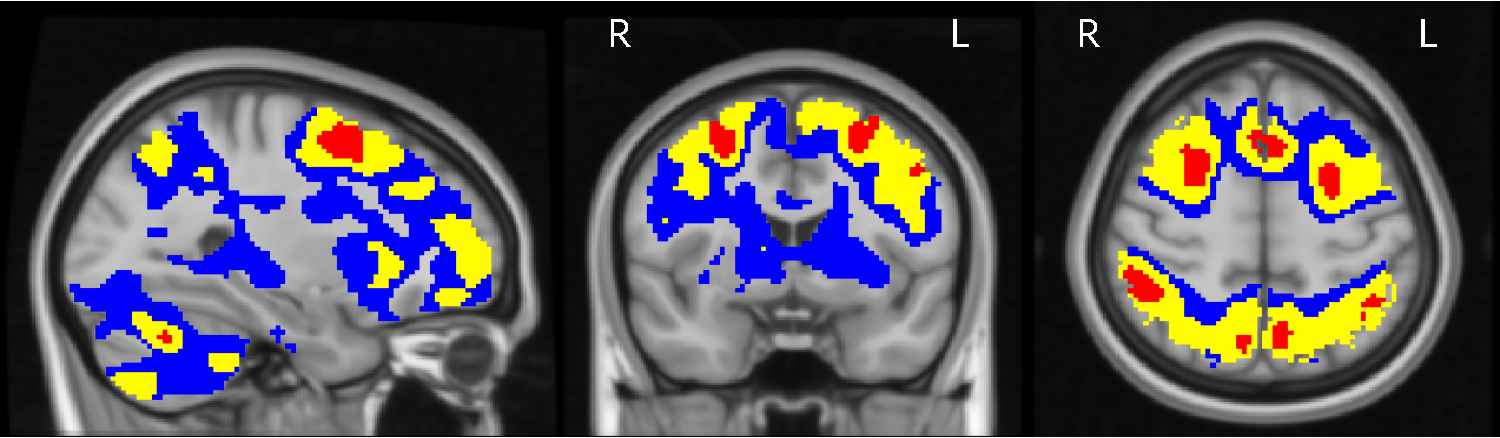
\includegraphics[height=45.5mm]{CIC_Fig1_Algorithm1_c05.pdf}\\
        0.8 Cohen's $d$ & 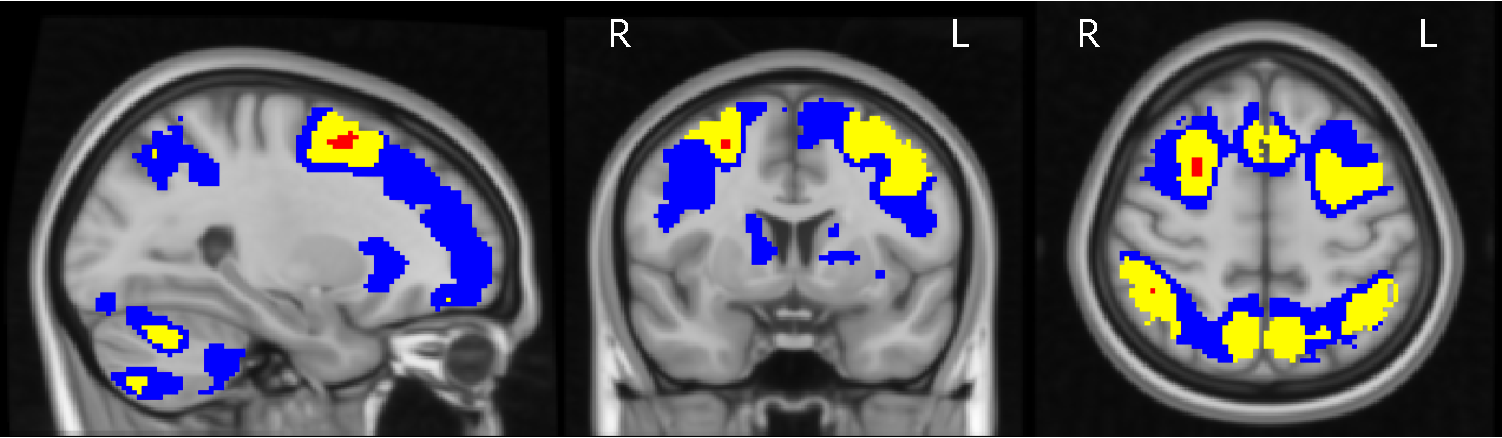
\includegraphics[height=45.5mm]{CIC_Fig1_Algorithm1_c08.pdf}\\
        1.2 Cohen's $d$ & 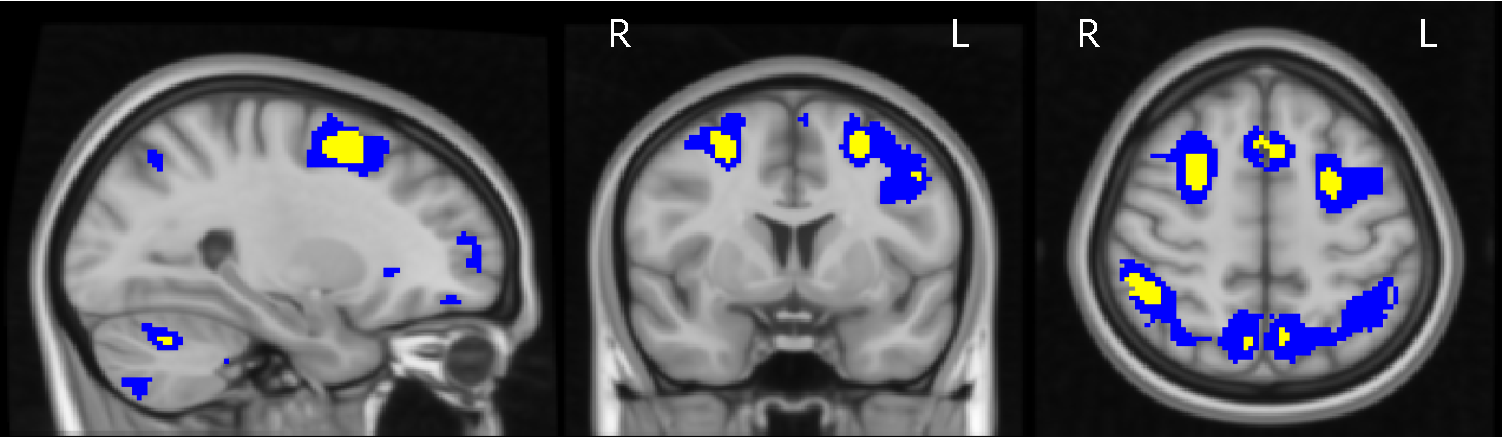
\includegraphics[height=45.5mm]{CIC_Fig1_Algorithm1_c12.pdf}\\
        \bottomrule
    \end{tabular}
\end{adjustbox}
    \captionof{figure}{Slices views of the Cohen's $d$ Confidence Sets obtained from applying Algorithm \ref{alg:one}.\ to the HCP working memory task data, using three Cohen's $d$ effect size thresholds, $c = 0.5, 0.8$ and $1.2$. Comparing with Fig.\ \ref{fig:HCP_Algorithm_3} and Fig.\ \ref{fig:HCP_Algorithm_2}, the CSs presented here are slightly more conservative than the corresponding CSs obtained with Algorithm \ref{alg:two}. and Algorithm \ref{alg:three}.\ (in the sense that the red upper CSs here are smaller, and blue lower CSs are larger). This is consistent with the simulation results obtained in Section \ref{sec:2D_sim_results} and \ref{sec:3d_sim_results}, where the empirical coverage for Algorithm \ref{alg:one}.\ was consistently larger than the other two methods.}
    \label{fig:HCP_Algorithm_1}
\end{table}

\begin{table}[!htbp]
\hspace*{-0.5cm}
\begin{adjustbox}{center}
\centering
    \begin{tabular}{cm{50mm}m{50mm}m{50mm}}
       \toprule
         Threshold $c$ & \hspace{1.4cm} Sagittal (X = 63) & \ \hspace{1.0cm} Coronal (Y = 130) & \hspace{0.9cm} Axial (Z = 124)\\
        \midrule
        0.5 Cohen's $d$ & 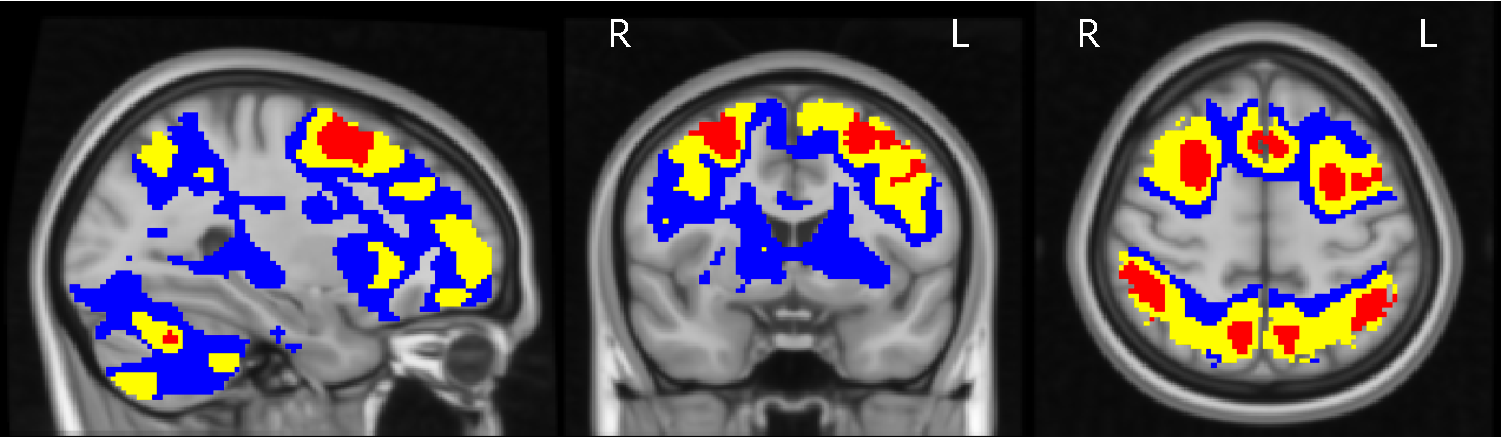
\includegraphics[height=45.5mm]{CIC_Fig1_Algorithm2_c05.pdf}\\
        0.8 Cohen's $d$ & 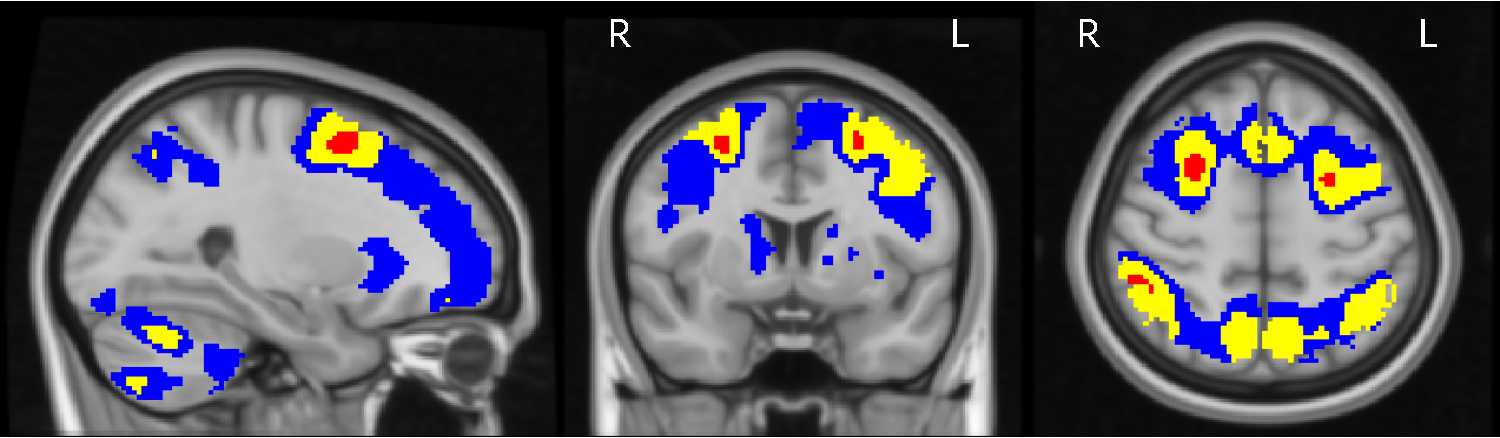
\includegraphics[height=45.5mm]{CIC_Fig1_Algorithm2_c08.pdf}\\
        1.2 Cohen's $d$ & 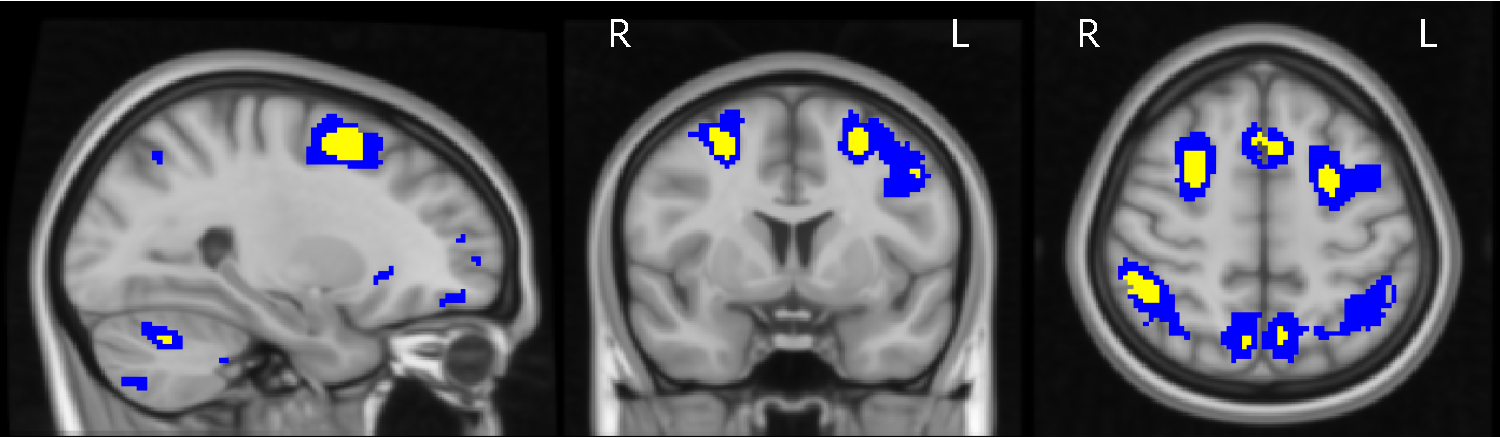
\includegraphics[height=45.5mm]{CIC_Fig1_Algorithm2_c12.pdf}\\
        \bottomrule
    \end{tabular}
\end{adjustbox}
    \captionof{figure}{Slices views of the Cohen's $d$ Confidence Sets obtained from applying Algorithm \ref{alg:two}.\ to the HCP working memory task data, using three Cohen's $d$ effect size thresholds, $c = 0.5, 0.8$ and $1.2$. Comparing with Fig.\ \ref{fig:HCP_Algorithm_3}, the upper and lower CSs presented here are almost identical to the corresponding CSs obtained with Algorithm \ref{alg:three}.}
    \label{fig:HCP_Algorithm_2}
\end{table}


\bibliographystyle{plainnat}
\bibliography{perm}        %% Start your bibliography here;
                                 %! with sample.bib as your bibliography file. You can
                               %% also use:
                %! \begin{thebibliography}
                %!    \bibitem{etc....
                %! \end{thebibliography}
                               %% to generate your bibliography.

%\begin{thesisauthorvita}             %% Write your vita here; it can be
%                                     %% anything in LaTeX2e par-mode.
%\end{thesisauthorvita}               %%

\end{document}                       %% Done.
